\documentclass[10pt, a4paper, italian]{article}
\usepackage[T1]{fontenc}
\usepackage[utf8]{inputenc}
\usepackage{amsmath, amssymb, amsthm, thmtools, amsfonts, mathtools}
\usepackage{nicefrac}
\usepackage{calc}
\usepackage[pdftex, hyperindex, plainpages=false]{hyperref}
\usepackage[nameinlink]{cleveref} %load before classicthesis (clash)
%\usepackage[nochapters,pdfspacing]{classicthesis}
\usepackage{siunitx}
\usepackage[siunitx]{circuitikz}

\usepackage[a4paper]{geometry}
\usepackage{float}
\usepackage{mdframed}
\usepackage{titling}
\usepackage{booktabs}
\usepackage{graphicx}
\usepackage{caption, subcaption}
\usepackage{xcolor}
\usepackage[italian]{babel}
\usepackage{pgfplots}
\usepackage{listings}
%\usepackage{lmodern}
\usepackage{url}
\usepackage{enumitem}
\usepackage{tikz} %loads after classicthesis (xcolor incompat)

% lets graphicx know path where figures to be included are found
\graphicspath{{../figs/}}
\makeatletter
\def\input@path{{../figs/}}
%or: \def\input@path{{/path/to/folder/}{/path/to/other/folder/}}
\makeatother

% tikz pgf plots setup
\usepgfplotslibrary{external}
\pgfplotsset{compat=1.15}
%\tikzexternalize

% spaces and significant digits/figures for measurements
\sisetup{free-standing-units, space-before-unit, number-unit-product = \;,
scientific-notation = false, round-mode = figures, round-precision = 1,}

% turns all (hyperlinked) references black [default is blue]
\hypersetup{
	linktoc=all,
	colorlinks=true,
	linkcolor=black
}

% code listings config
%\lstset{
%language=Python,
%basicstyle=\ttfamily,
%columns=fullflexible,
%keepspaces=true,
%}

% mdframed (for boxed text) configuration
\mdfsetup{linewidth=0.6pt}

% Default fixed font does not support bold face
\DeclareFixedFont{\ttb}{T1}{txtt}{bx}{n}{12} % for bold
\DeclareFixedFont{\ttm}{T1}{txtt}{m}{n}{12}  % for normal

% Custom colors
\usepackage{color}
\definecolor{deepblue}{rgb}{0,0,0.5}
\definecolor{deepred}{rgb}{0.6,0,0}
\definecolor{deepgreen}{rgb}{0,0.5,0}

% Commands 
\newcommand{\executeiffilenewer}[3]{%
	\ifnum\pdfstrcmp{\pdffilemoddate{#1}}%
		{\pdffilemoddate{#2}}>0%
	{\immediate\write18{#3}}\fi%
}
% input .svg --> .pdf_tex graphs
%\newcommand{\includesvg}[1]{%
%	\executeiffilenewer{#1.svg}{#1.pdf}%
%	{inkscape -z -D --file=#1.svg %
%	--export-pdf=#1.pdf --export-latex}%
%	\input{#1.pdf_tex}%
%}
% Thanks UniPi's Department of Physics E. Fermi
\newcommand{\thanksdf}{(\thanks{Dipartimento di Fisica E.~Fermi,%
Universit\`a di Pisa - Pisa, Italy.}\;)}

% hyperlink to email address
\newcommand{\mail}[1]{\href{mailto:#1}{\textsf{#1}}}

% \vec for bold vectors, instead of overarrows (now "\arrvec")
\let\arrvec=\vec
\renewcommand{\vec}[1]{\boldsymbol #1}
% replaces straight phi with slanted phi
\renewcommand{\phi}{\varphi}
% replaces straight eps with curved epsilon
\newcommand{\eps}{\varepsilon}
% abbreviation for (sub_/super^)scripts of \lim, \sum,... in inline math
\newcommand{\ds}{\displaystyle}

% blackboard/number set letters
\newcommand{\CC}{\mathbb C}
\newcommand{\HH}{\mathbb H}
\newcommand{\KK}{\mathbb K}
\newcommand{\NN}{\mathbb N}
\newcommand{\PP}{\mathbb P}
\newcommand{\QQ}{\mathbb Q}
\newcommand{\RR}{\mathbb R}
\newcommand{\ZZ}{\mathbb Z}

\newcommand{\Abs}[1]{{\left\Vert #1\right\Vert}}
\newcommand{\enclose}[1]{{\left( #1 \right)}}
\newcommand{\Enclose}[1]{{\left[ #1 \right]}}
\newcommand{\floor}[1]{\left\lfloor #1 \right\rfloor}
\newcommand{\ceil}[1]{\left\lceil #1 \right\rceil}
\newcommand{\To}{\rightrightarrows}

% Math operators
\DeclareMathOperator{\divergence}{div}
\renewcommand{\div}{\divergence}
\DeclareMathOperator{\Imaginarypart}{Im}
\renewcommand{\Im}{\Imaginarypart}
\DeclareMathOperator{\Realpart}{Re}
\renewcommand{\Re}{\Realpart}
%\DeclareMathOperator{\arg}{arg}
\DeclareMathOperator{\tg}{tg}
\DeclareMathOperator{\arctg}{arctg}
\DeclareMathOperator{\settsinh}{settsinh}
\DeclareMathOperator{\settcosh}{settcosh}
\DeclareMathOperator{\tr}{tr}
\DeclareMathOperator{\im}{im}
\DeclareMathOperator{\sgn}{sgn}
\DeclareMathOperator{\diag}{diag}

\DeclarePairedDelimiter{\norm}{\lVert}{\rVert}
\DeclarePairedDelimiter{\scalar}{\langle}{\rangle}

% Logarithm with arbitrary base.
% -> log_10
\newcommand{\llog}[1][10]{\log_{#1}}

% Absolute value.
% -> |x|
\newcommand{\abs}[1]{\left| #1 \right|}

% Powers.
% -> x^a
\newcommand{\power}[2][2]{\left( #2 \right)^{#1}}

% Square.
% -> x^2
\newcommand{\sq}[1]{\power[2]{#1}}

% Expansion of the binomial coefficient.
% -> n1!/(n2!(n1 - n2)!)
\newcommand{\binomexpr}[2]{\frac{#1!}{#2!(#1 - #2)!}}

% Expression evaluation at a given point with square brackets.
% -> [x]_{a}
\newcommand{\at}[2]{\left[ #1\right]_{\makebox[-1pt][l]{${\scriptstyle#2}$}}}

% Expression evaluation in an interval.
% -> [x] _{a}^{b}
\newcommand{\eval}[3]{\left.#1%
  \right|_{\makebox[-1pt][l]{${\scriptstyle#2}$}}^{\makebox[-1pt][l]{${\scriptstyle#3}$}}}

% Upright d in math mode (for differentials).
% -> d
\newcommand{\ud}{\mathrm{d}}

% Differential.
% -> dx
\newcommand{\diff}[1][x]{\,\ud{#1}}

% Base command for defining derivatives.
% -> df/dx or d^kf/dx^k
\newcommand{\basederivative}[4][]{%
  \displaystyle%
  \ifx\\#1\\\frac{#4#2}{#4#3}%
  \else%
  \frac{#4^#1#2}{#4#3^#1}%
  \fi%
}

% Total derivative.
% -> df/dx(x) or d^kf/dx^k(x)
\newcommand{\td}[4][]{%
  \basederivative[#1]{#2}{#3}{\ud}%
  \ifx\\#4\\%
  \else%
  \mkern-4mu\left(#4\right)%
  \fi%
}

% Partial derivative.
% -> df/dx(x) or d^kf/dx^k(x)
\newcommand{\pd}[4][]{%
  \basederivative[#1]{#2}{#3}{\partial}%
  \ifx\\#4\\%
  \else%
  \mkern-4mu\left(#4\right)%
  \fi%
}

\newcommand{\intinf}{\int_{-\infty}^{\infty}\!\!\!}

\newcommand{\cinterval}[2]{\left[\, #1,~#2 \,\right]}

\newcommand{\linterval}[2]{\left[\, #1,~#2 \,\right)}

\newcommand{\rinterval}[2]{\left(\, #1,~#2 \,\right]}

\newcommand{\ointerval}[2]{\left(\, #1,~#2 \,\right)}

\newcommand{\prob}[1]{\displaystyle P\left(#1\right)}

\newcommand{\pvalue}{\emph{$p$-value}}

\newcommand{\cond}{\,|\,}

\newcommand{\expect}[1]{\displaystyle E\left[#1\right]}

\newcommand{\mom}[2][]{\displaystyle {\cal M}_{#2}\ifx\\#1\\\else(#1)\fi}

\newcommand{\momalg}[1]{\displaystyle \lambda_{#1}}

\newcommand{\momcen}[1]{\displaystyle \mu_{#1}}

\newcommand{\skewness}{\displaystyle \gamma_1}

\newcommand{\kurtosis}{\displaystyle \gamma_2}

\newcommand{\charf}[1][x]{\phi_{#1}}

\newcommand{\momgenf}[1][x]{M_{#1}}

\newcommand{\fwhm}{{\scriptstyle \textsc{FWHM}}}

\newcommand{\hwhm}{{\scriptstyle \textsc{HWHM}}}

\newcommand{\median}{\mu_{\nicefrac{1}{2}}}

\newcommand{\var}[1]{\ensuremath{\text{Var}\left(#1\right)}}

\newcommand{\cov}[2]{\ensuremath{\text{Cov}\left(#1, #2\right)}}

\newcommand{\corr}[2]{\ensuremath{\text{Corr}\left(#1, #2\right)}}

\newcommand{\like}{\mathcal L}

\newcommand{\likelihood}[2][]{\like\ifx\\#2\\\else(#2\ifx\\#1\\\else;#1\fi)\fi}

\newcommand{\chisq}{\ensuremath{\chi^2}}

\newcommand{\chisquare}[2][]{\chisq\ifx\\#2\\\else(#2\ifx\\#1\\\else;#1\fi)\fi}

\newcommand{\loglikelihood}[2][]{\log\likelihood[#1]{#2}}

\newcommand{\pdf}[3][]{#2(#3\ifx\\#1\\\else;#1\fi)}

\newcommand{\binomialpdf}[2][]{\pdf[#1]{\mathcal B}{#2}}

\newcommand{\multinomialpdf}[2][]{\pdf[#1]{\mathcal M}{#2}}

\newcommand{\poissonpdf}[2][]{\pdf[#1]{\mathcal P}{#2}}

\newcommand{\uniformpdf}[2][]{\pdf[#1]{u}{#2}}

\newcommand{\exponentialpdf}[2][]{\pdf[#1]{\varepsilon}{#2}}

\newcommand{\gausspdf}[2][]{\pdf[#1]{N}{#2}}

\newcommand{\chisquarepdf}[2][]{\pdf[#1]{\wp}{#2}}

\newcommand{\cauchypdf}[2][]{\pdf[#1]{c}{#2}}

\newcommand{\erf}[1]{\ensuremath{\text{erf}\left(#1\right)}}

\newcommand{\dccases}[4][]{#2 \ifx\\#2\\\else=\fi %
  \begin{cases}
    \displaystyle #3 & \text{per variabili discrete}\\
    \displaystyle #4 & \text{per variabili continue}#1
  \end{cases}
}
% sub/super-scriptable for all symbol as math operator 
\newcommand\Scaleforall[1]{\vcenter{\hbox{\scalefont{#1}$\forall$}}}

\DeclareMathOperator*\forevery{%
  \vphantom\sum
  \mathchoice{\Scaleforall{2}}{\Scaleforall{1.4}}{\Scaleforall{1}}{\Scaleforall{0.75}}}
\usepackage{multicol}
\geometry{left=2cm, right=2cm, top=2cm, bottom=2cm}
\usepackage{colortbl}
\usepackage{diagbox}
\usepackage[T1]{fontenc}
\usepackage[utf8]{inputenc}
\usepackage{graphicx}
\usepackage{xcolor}
\usepackage{tkz-graph}
\usepackage{arydshln}
\usetikzlibrary{automata, positioning, arrows}
\newenvironment{FSM}{
\begin{tikzpicture}
\tikzset{
->, % makes the edges directed
>=stealth', % makes the arrow heads bold
node distance=2cm, % specifies the minimum distance between two nodes. Change if necessary.
every state/.style={minimum size = 1cm, thick, fill=gray!10}, % sets the properties for each 'state' node
}
}{
\end{tikzpicture}
}


\lstset{%
  language = Octave,
  backgroundcolor=\color{white},   
  basicstyle=\footnotesize\ttfamily,       
  breakatwhitespace=false,         
  breaklines=true,                 
  captionpos=b,                   
  commentstyle=\color{gray},    
  deletekeywords={...},           
  escapeinside={\%*}{*)},          
  extendedchars=true,              
  frame=single,                    
  keepspaces=true,                 
  keywordstyle=\color{orange},       
  morekeywords={*,...},            
  numbers=left,                    
  numbersep=5pt,                   
  numberstyle=\footnotesize\color{gray}, 
  rulecolor=\color{black},         
  rulesepcolor=\color{blue},
  showspaces=false,                
  showstringspaces=false,          
  showtabs=false,                  
  stepnumber=2,                    
  stringstyle=\color{orange},    
  tabsize=2,                       
  title=\lstname,
  emphstyle=\bfseries\color{blue}%  style for emph={} 
} 

%% language specific settings:
\lstdefinestyle{Arduino}{%
    language = Octave,
    keywords={void, int boolean},%                 define keywords
    morecomment=[l]{//},%             treat // as comments
    morecomment=[s]{/*}{*/},%         define /* ... */ comments
    emph={HIGH, OUTPUT, LOW}%        keywords to emphasize
}

% indexes subsections with letters, sections with numbers (1.a, 1.b, ...)
\renewcommand{\thesubsection}{\thesection.\alph{subsection}}

% lets graphicx know path where figures to be included are found
\graphicspath{{../figs/}}

\newcommand{\dontcare}{X}
\author{Gruppo 1.AC \\ Matteo Rossi, Bernardo Tomelleri}
\title{EsD4 ADC-DAC: Convertitore sigma-delta}
\begin{document}
\date{\today}
\maketitle

\section*{Misura componenti dei circuiti}
Riportiamo per completezza il valore della tensione continua di
alimentazione per i circuiti integrati misurata con il multimetro
\begin{align*}
V_{CC} &= 4.99 \pm 0.03 \si{\V} \\
V_{EE} &= -4.99 \pm 0.03 \si{\V}
\end{align*}
e i valori di capacità dei condensatori di disaccoppiamento che collegano le
linee di alimentazione a massa (sempre misurato con il multimetro)
\begin{align*}
C_{d+} &= 97 \pm 4 \; \si{n\F} \\
C_{d-} &= 107 \pm 4 \; \si{n\F}
\end{align*}

Abbiamo inoltre misurato i valori dei vari componenti del circuito:
\begin{tabular}{cccccc}
\toprule
Resistenze $[\si{\ohm}]$ & $R$ & $\sigma R$ & Capacità $[\si{n\F}]$ & $C$ &
$\sigma C$ \\
\midrule
\midrule
$R_1$	  	& 996 	& 8		& $C_1$ & 94	& 4 \\
$R_2$	  	& 994	& 8		& & & \\
$R_3$	  	& 999	& 8		& & & \\
$R_4$	  	& 994 	& 8	& & & \\
$R_5$	  	& 997	& 8 & & & \\

\bottomrule   
\end{tabular}
\caption{Valori di resistenza e capacità misurate per i componenti del primo
circuito studiato.}
\end{table}
\begin{tabular}{cccccc}
\toprule
Resistenze $[\si{\ohm}]$ & $R$ & $\sigma R$ & Capacità $[\si{n\F}]$ & $C$ &
$\sigma C$ \\
\midrule
\midrule
$R_1$	  	& 995 	& 8		& $C_1$ & 109	& 4 \\
$R_2$	  	& 999	& 8		& & & \\
$R_3$	  	& 998	& 8		& & & \\
$R_4$	  	& 998 	& 8	& & & \\
$R_5$	  	& 996	& 8 & & & \\

\bottomrule   
\end{tabular}
\caption{Valori di resistenza e capacità misurate per i componenti del secondo
circuito studiato.}
\end{table}
\setcounter{section}{0}

%=======================
\section{Analisi e costruzione del circuito}\label{sec: IC}
\begin{figure}[htbp]
    \centering
	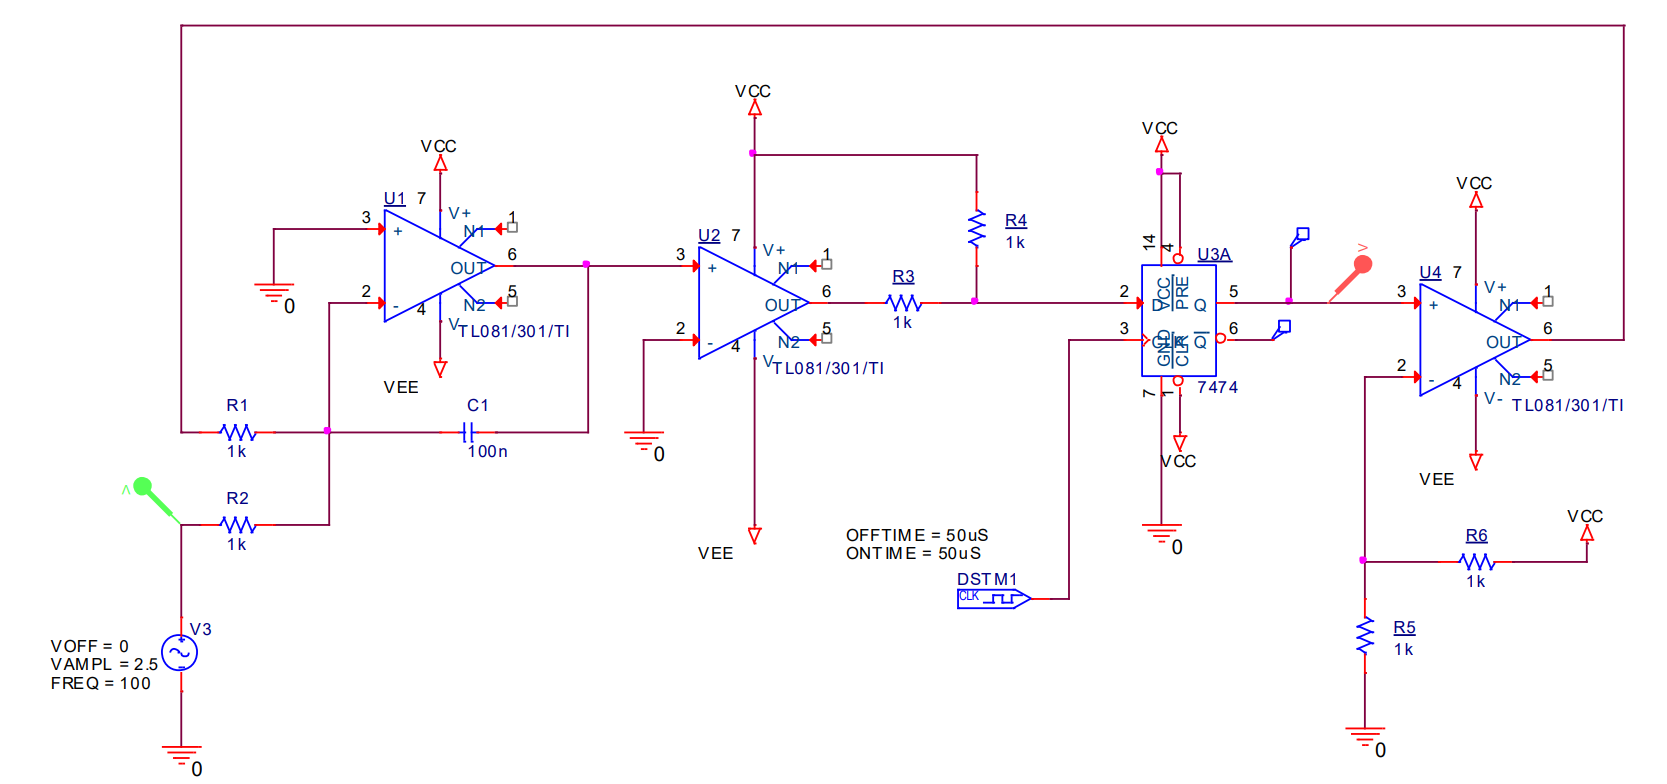
\includegraphics[width=\textwidth]{schem}
    \caption{Schematica del circuito utilizzato per il convertitore analogico digitale}
\end{figure}
\subsection{Verifica del funzionamento}
\begin{figure}[htbp]
    \centering
	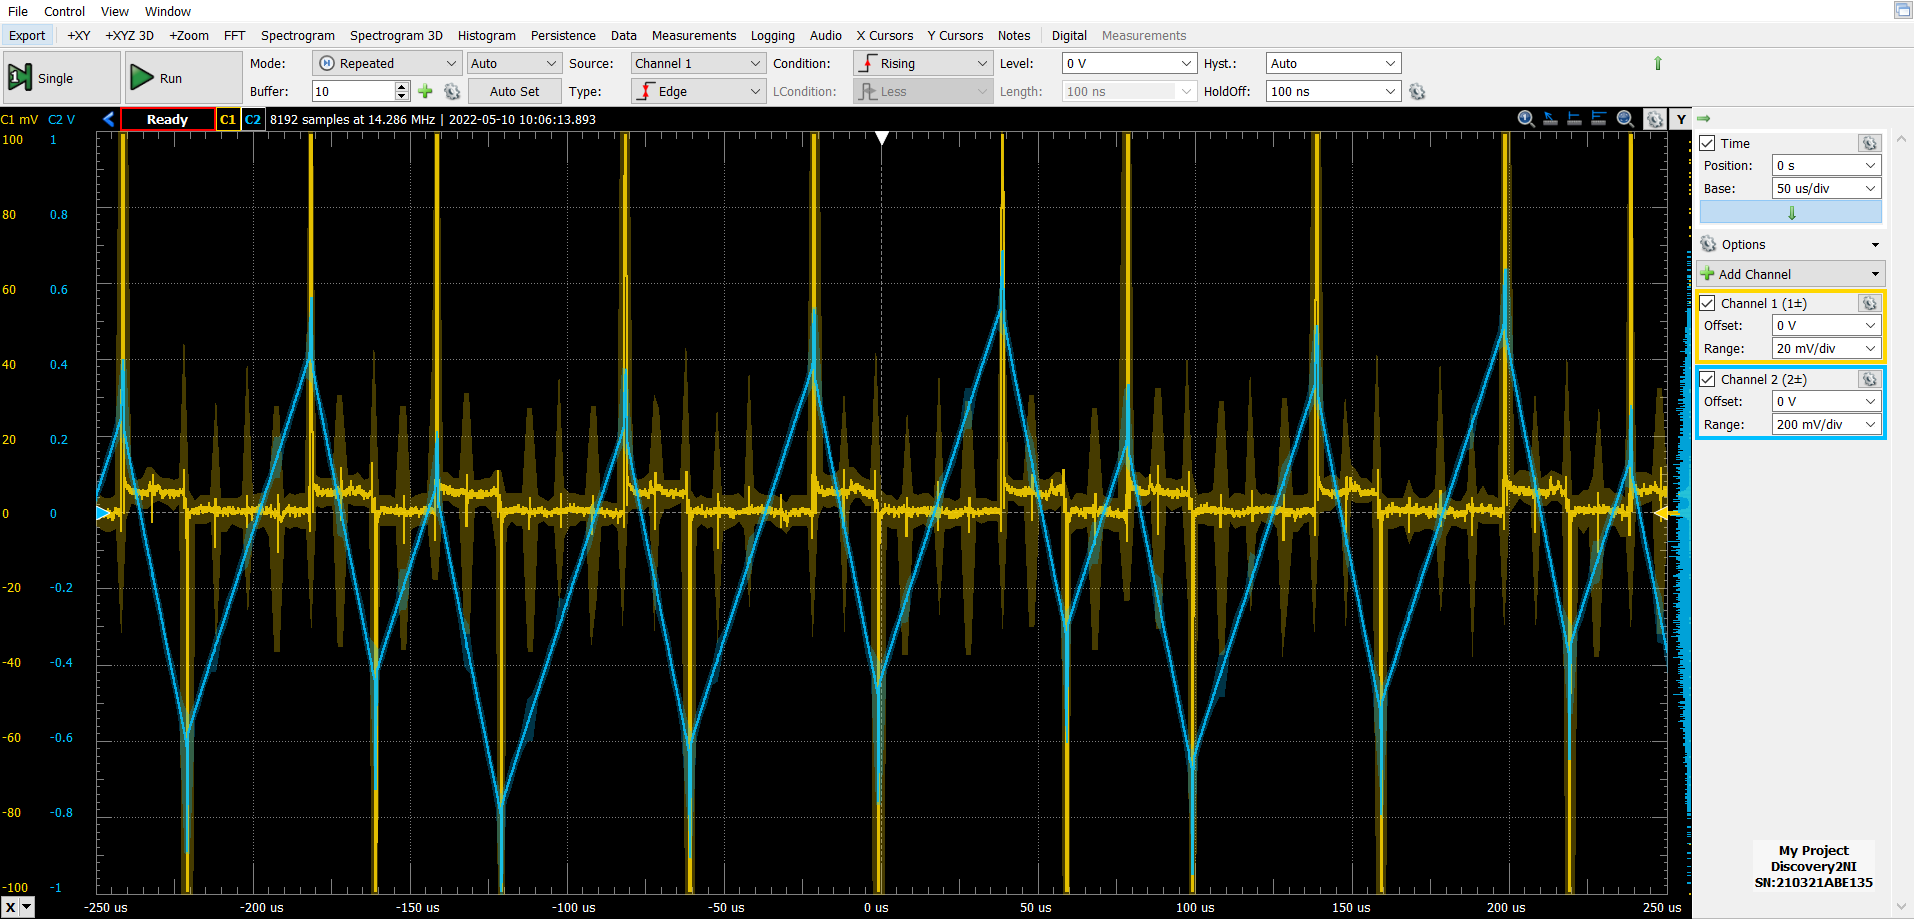
\includegraphics[width=\textwidth]{MIDDLE.U1.InputVSOutput}
    \caption{Acquisizione del segnale nell'ingresso invertente (canale 1) e dell'uscita (canale 2) del circuito integratore}
\end{figure}
\begin{figure}[htbp]
    \centering
	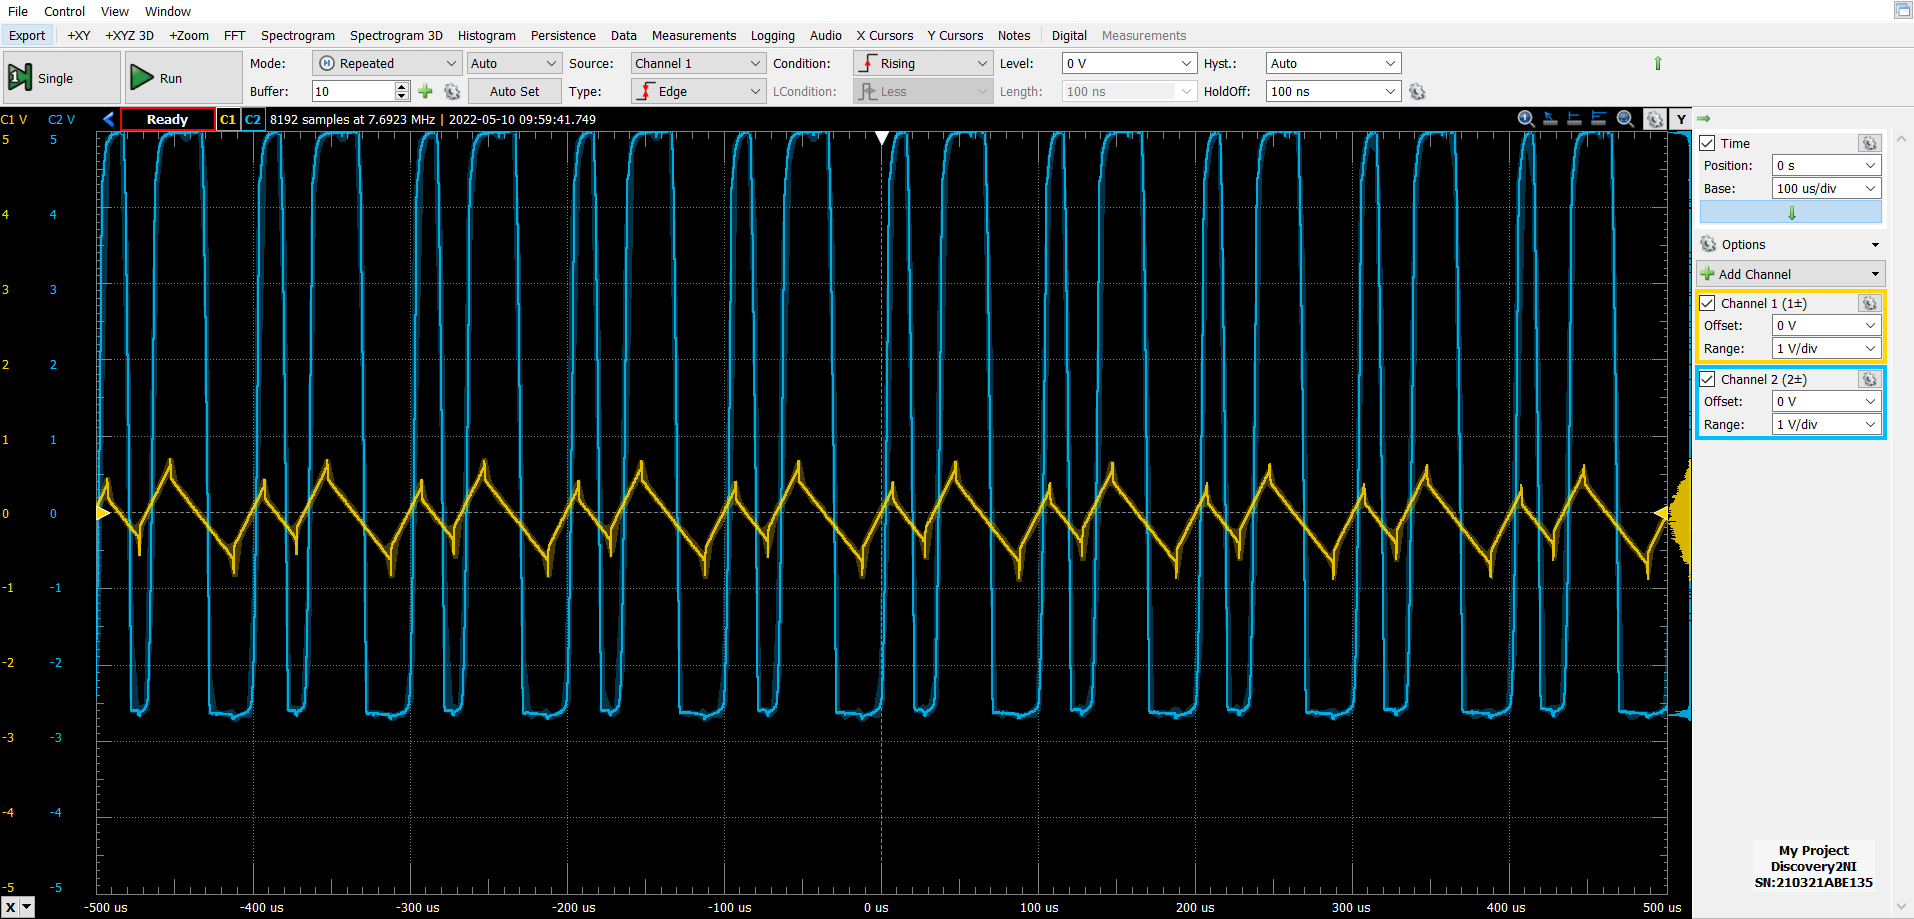
\includegraphics[width=\textwidth]{MIDDLE.U2.InputVSOutput}
    \caption{Acquisizione del segnale nell'ingresso non invertente (canale 1) e dell'uscita (canale 2) del circuito comparatore semplice}
\end{figure}
\begin{figure}[htbp]
    \centering
	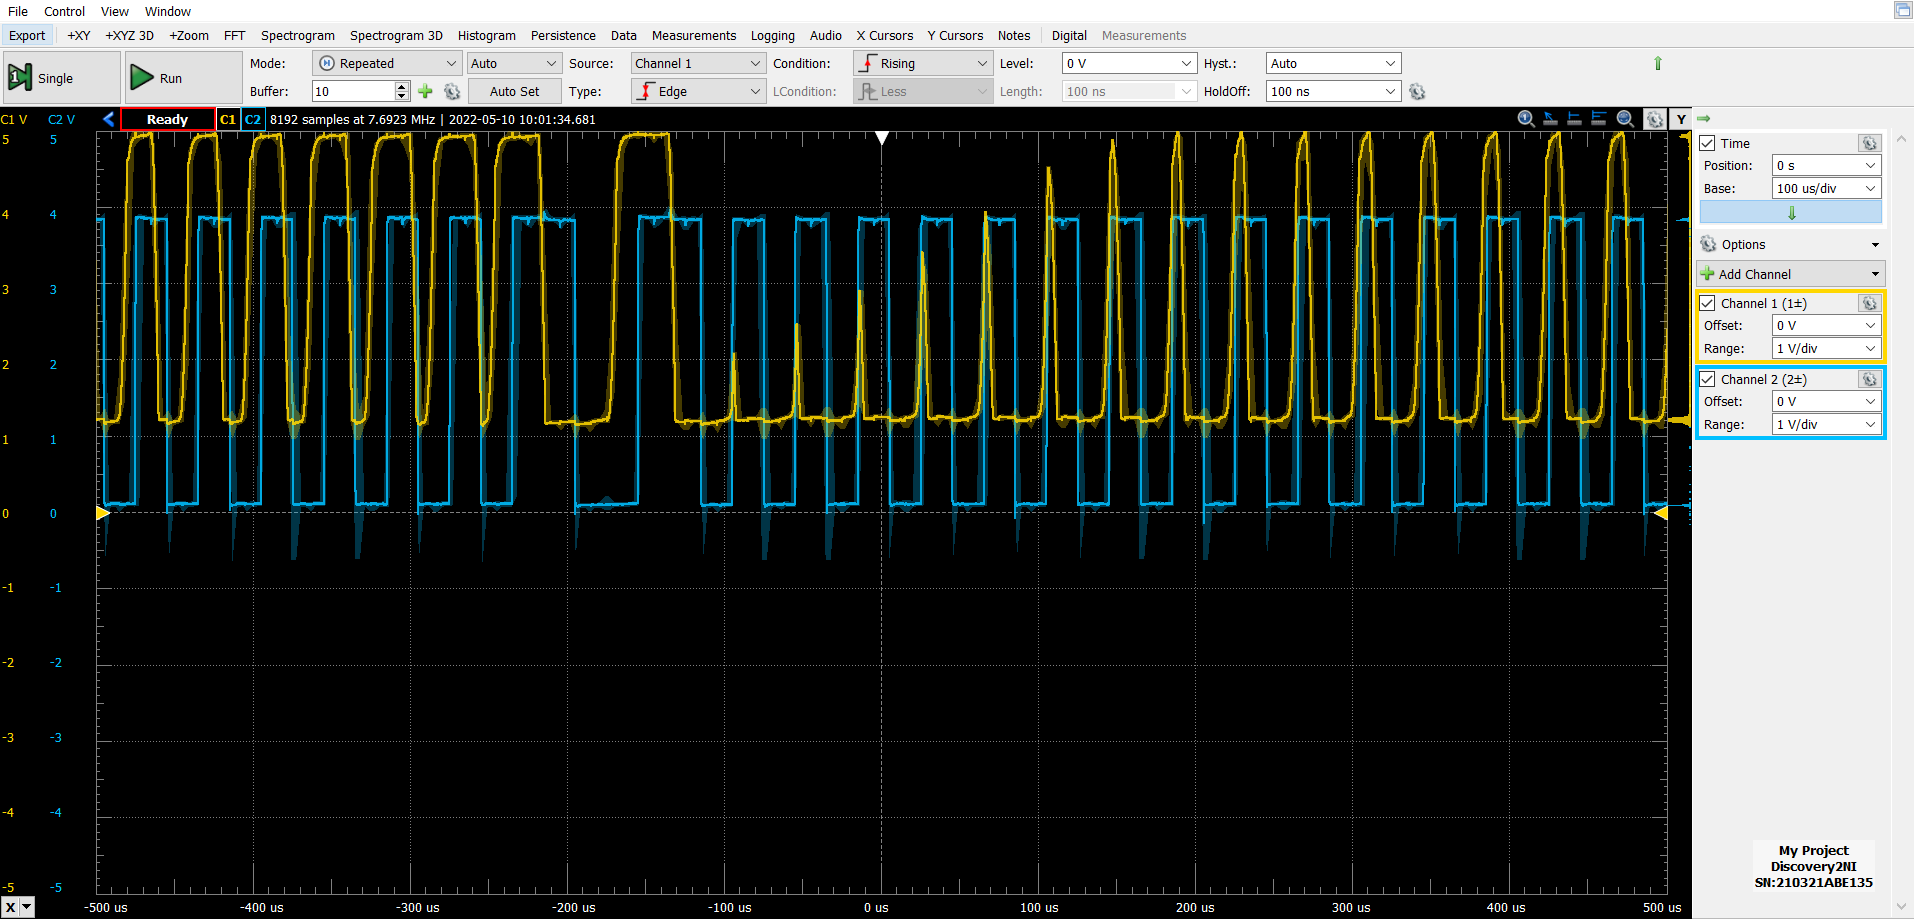
\includegraphics[width=\textwidth]{MIDDLE.U3.InputVSOutput}
    \caption{Acquisizione del segnale in ingresso(canale 1) e in uscita (canale 2) dal Flip Flop}
\end{figure}
\begin{figure}[htbp]
    \centering
	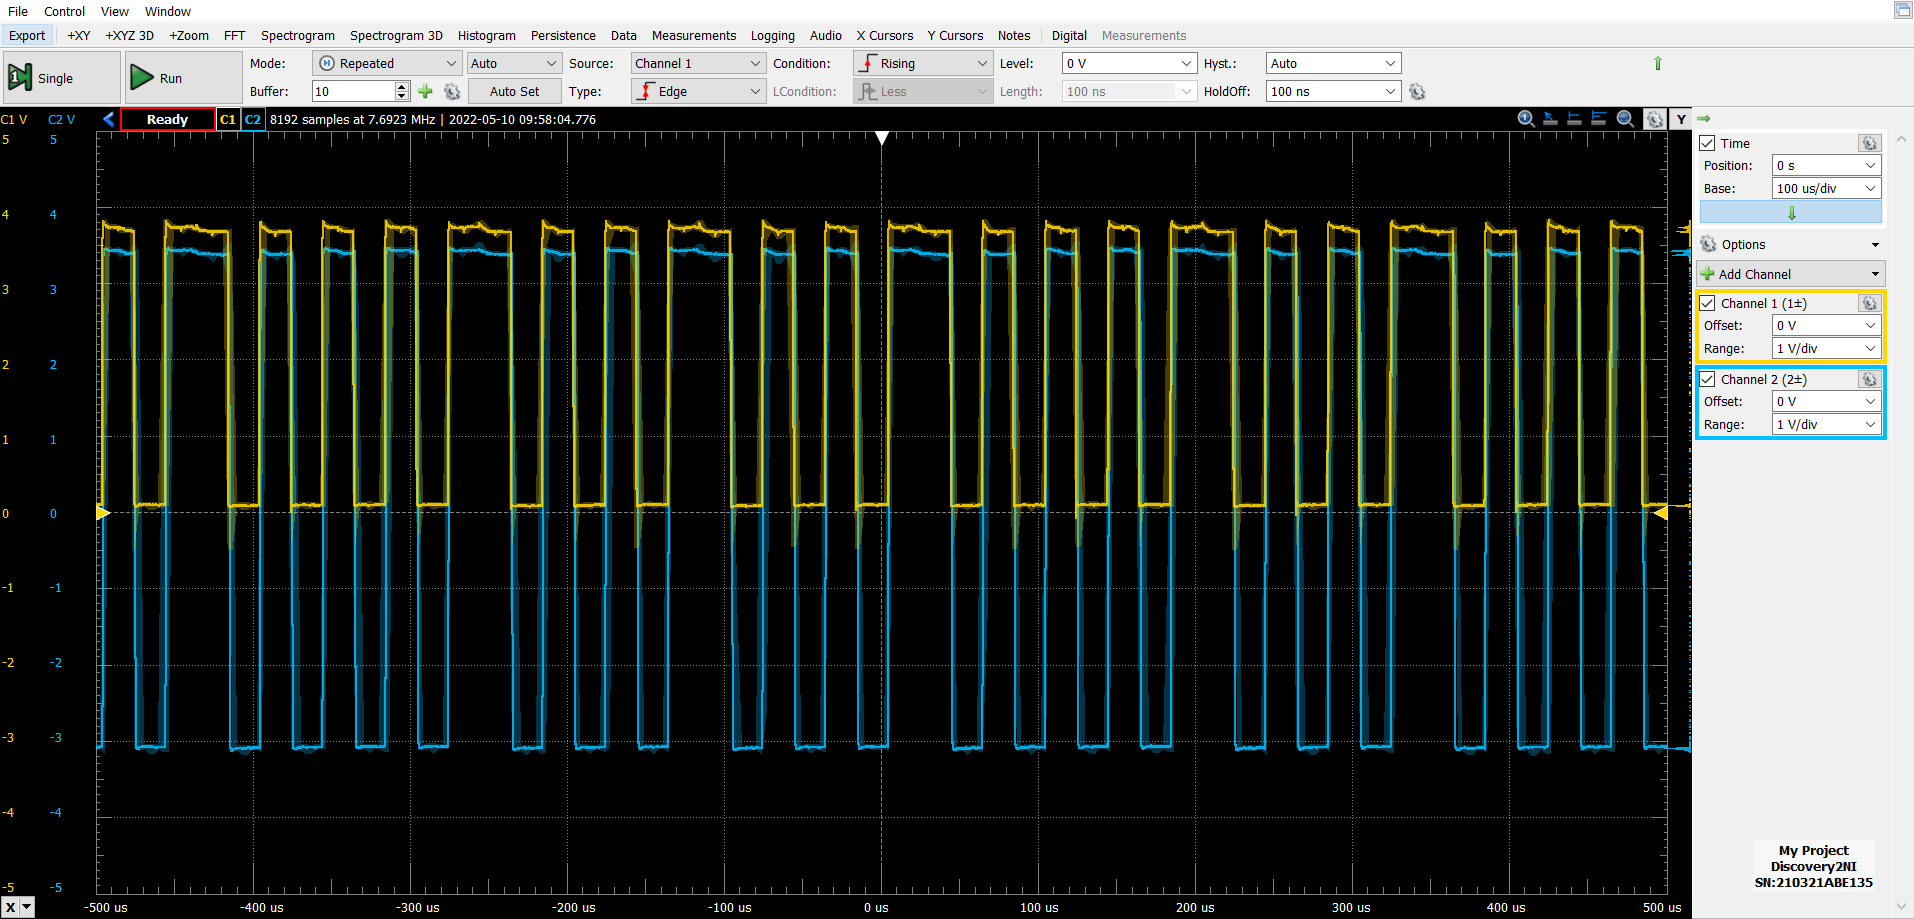
\includegraphics[width=\textwidth]{MIDDLE.U3vU4}
    \caption{Acquisizione del segnale in uscita dal pin Q del Flip Flop(canale 1) e in uscita dal DAC (canale 2)}
\end{figure}

\begin{figure}[htbp]
    \centering
	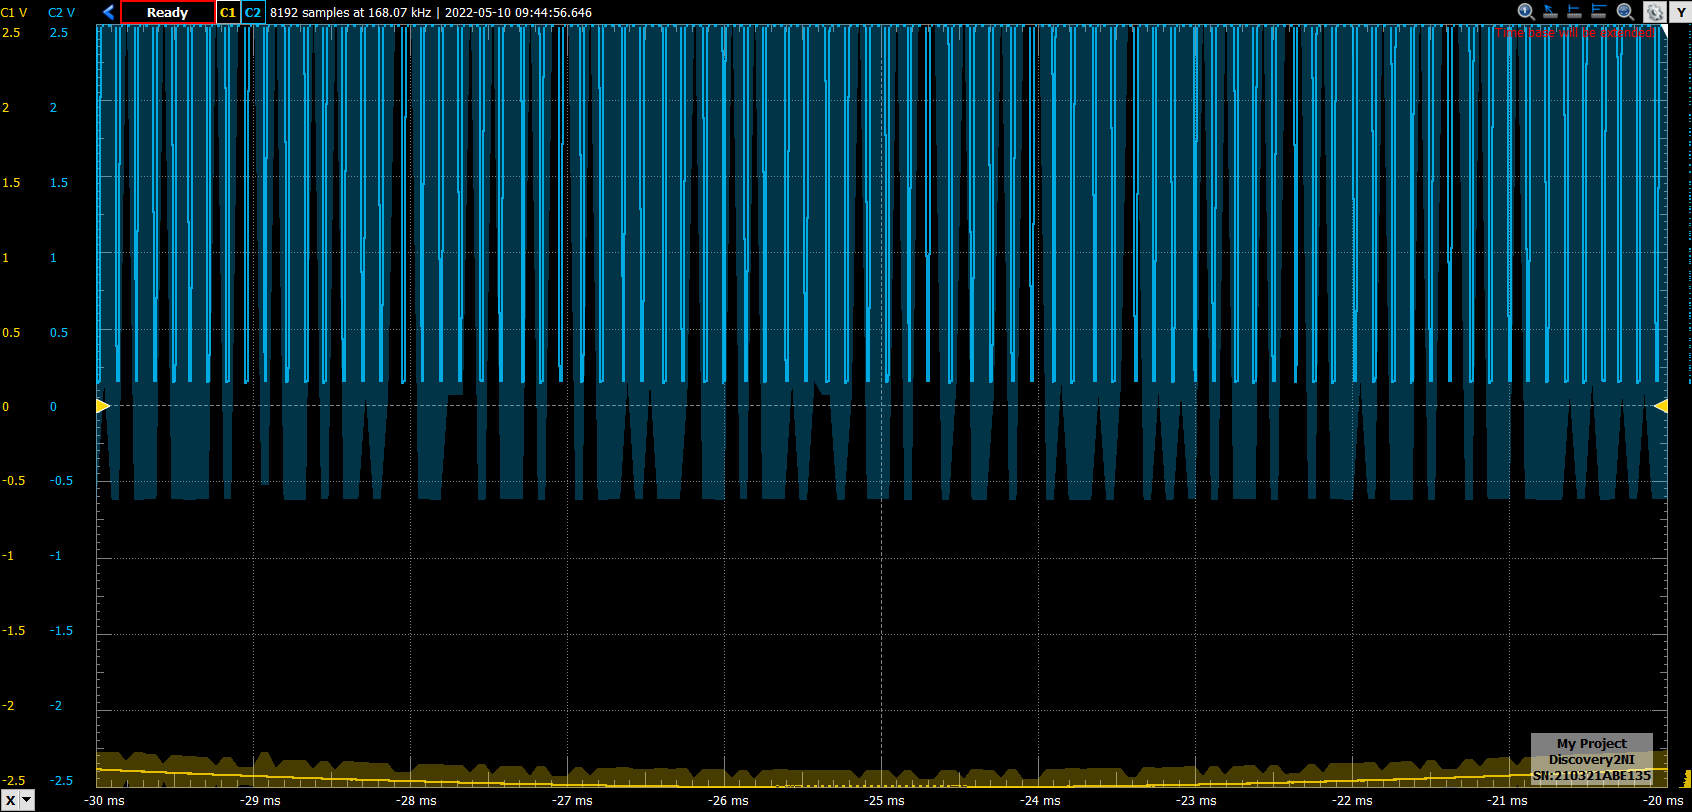
\includegraphics[width=\textwidth]{BOTTOM}
    \caption{Acquisizione del segnale analogico in ingresso (un'onda sinusoidale di frequenza pari a 10 Hz e ampiezza pari a $2.5 V$) e del segnale logico in uscita dal pin Q del Flip-Flop durante il minimo del segnale}
\end{figure}
\begin{figure}[htbp]
    \centering
	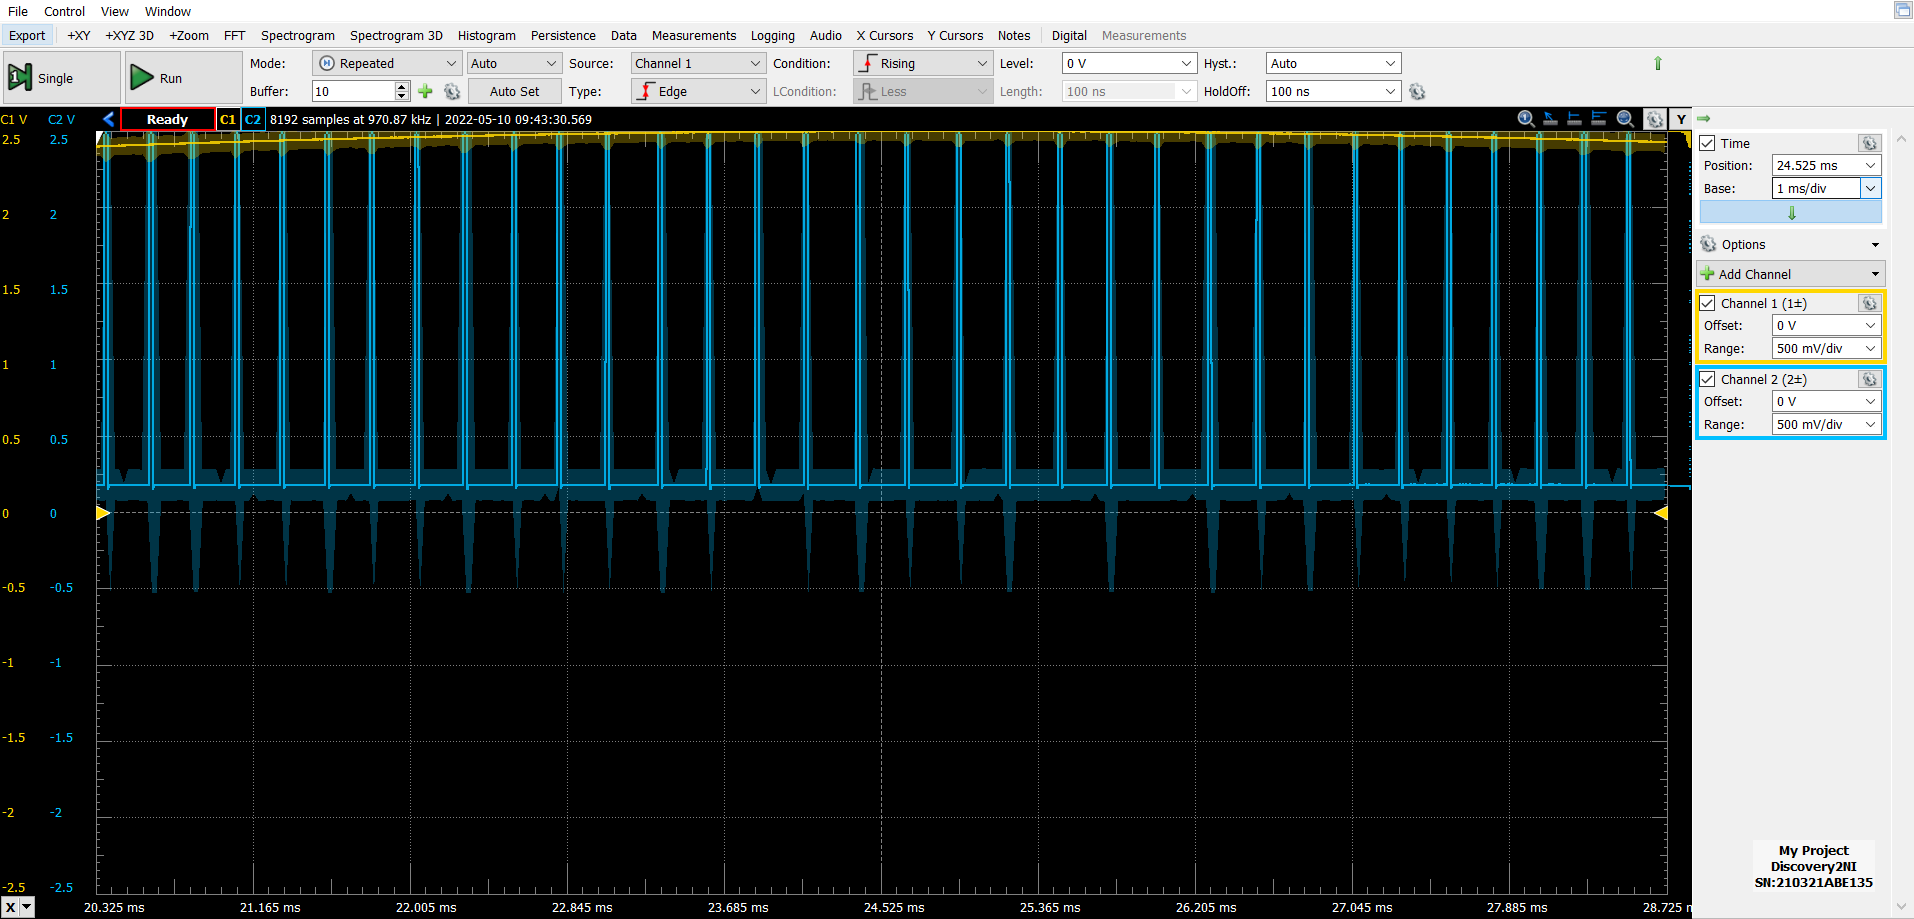
\includegraphics[width=\textwidth]{TOP}
    \caption{Acquisizione del segnale analogico in ingresso (un'onda sinusoidale di frequenza pari a 10 Hz e ampiezza pari a $2.5 V$) e del segnale logico in uscita dal pin Q del Flip-Flop durante il massimo del segnale}
\end{figure}
\begin{figure}[htbp]
    \centering
	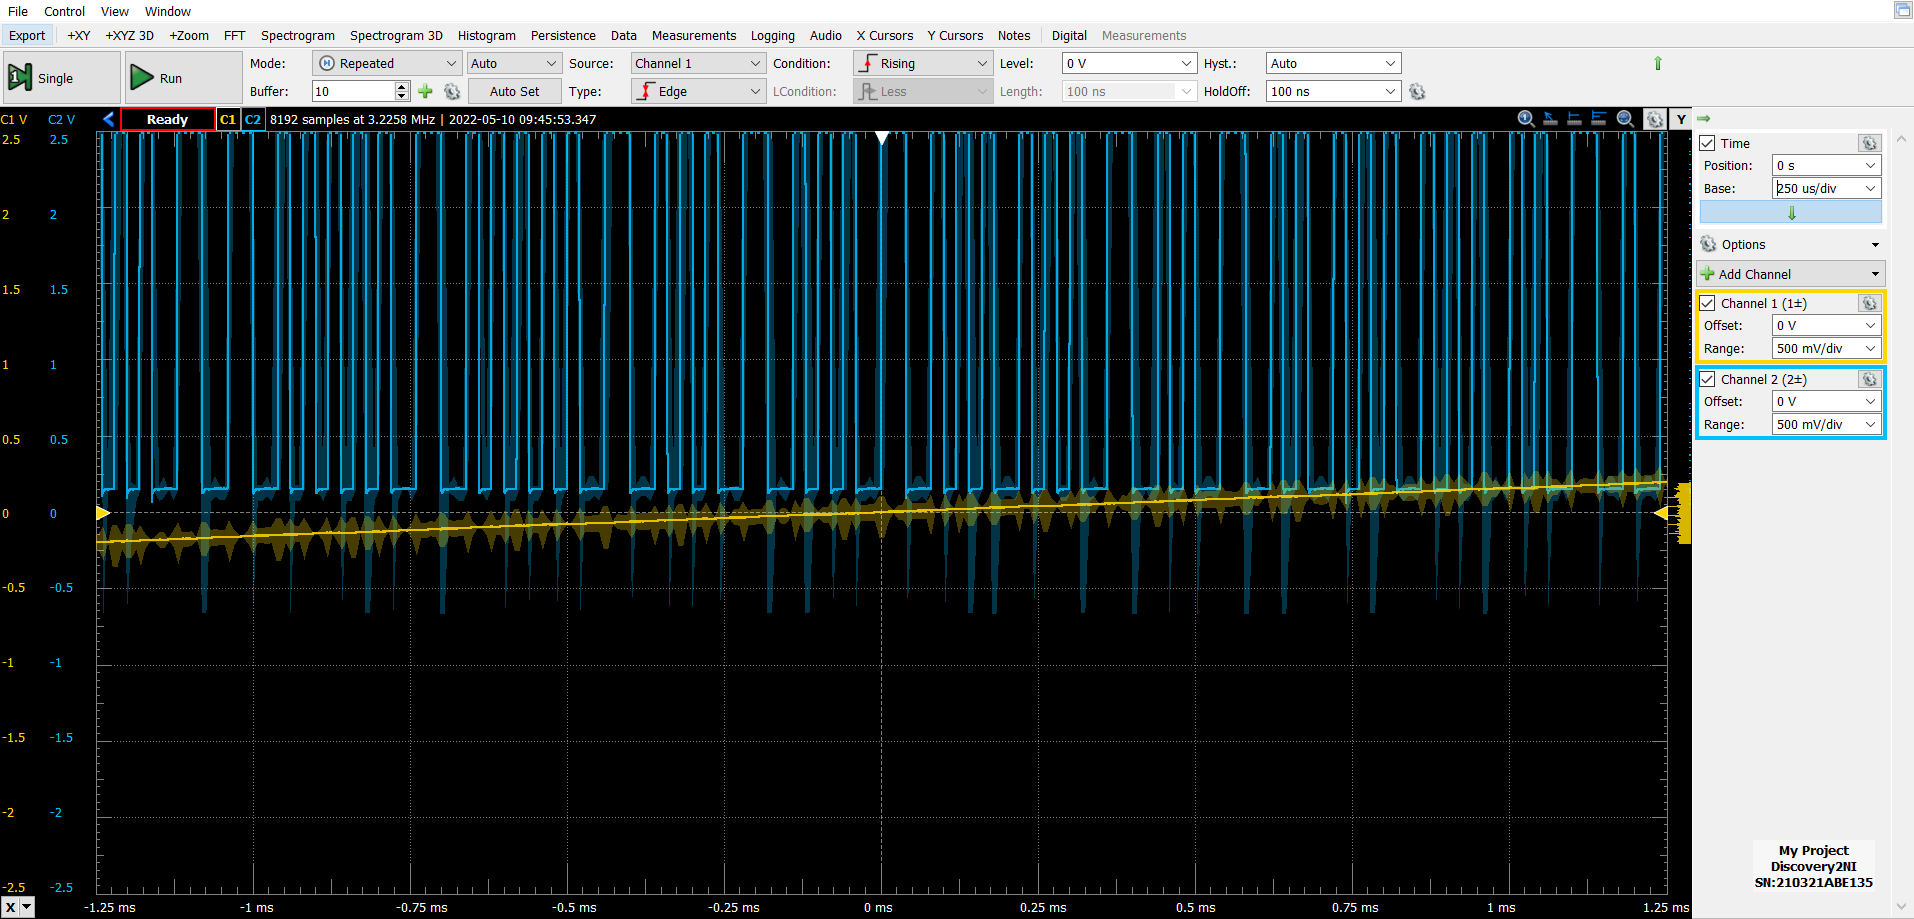
\includegraphics[width=\textwidth]{MIDDLE}
    \caption{Acquisizione del segnale analogico in ingresso (un'onda sinusoidale di frequenza pari a 10 Hz e ampiezza pari a $2.5 V$) e del segnale logico in uscita dal pin Q del Flip-Flop durante il punto medio dell'onda}
\end{figure}
\begin{figure}[htbp]
    \centering
	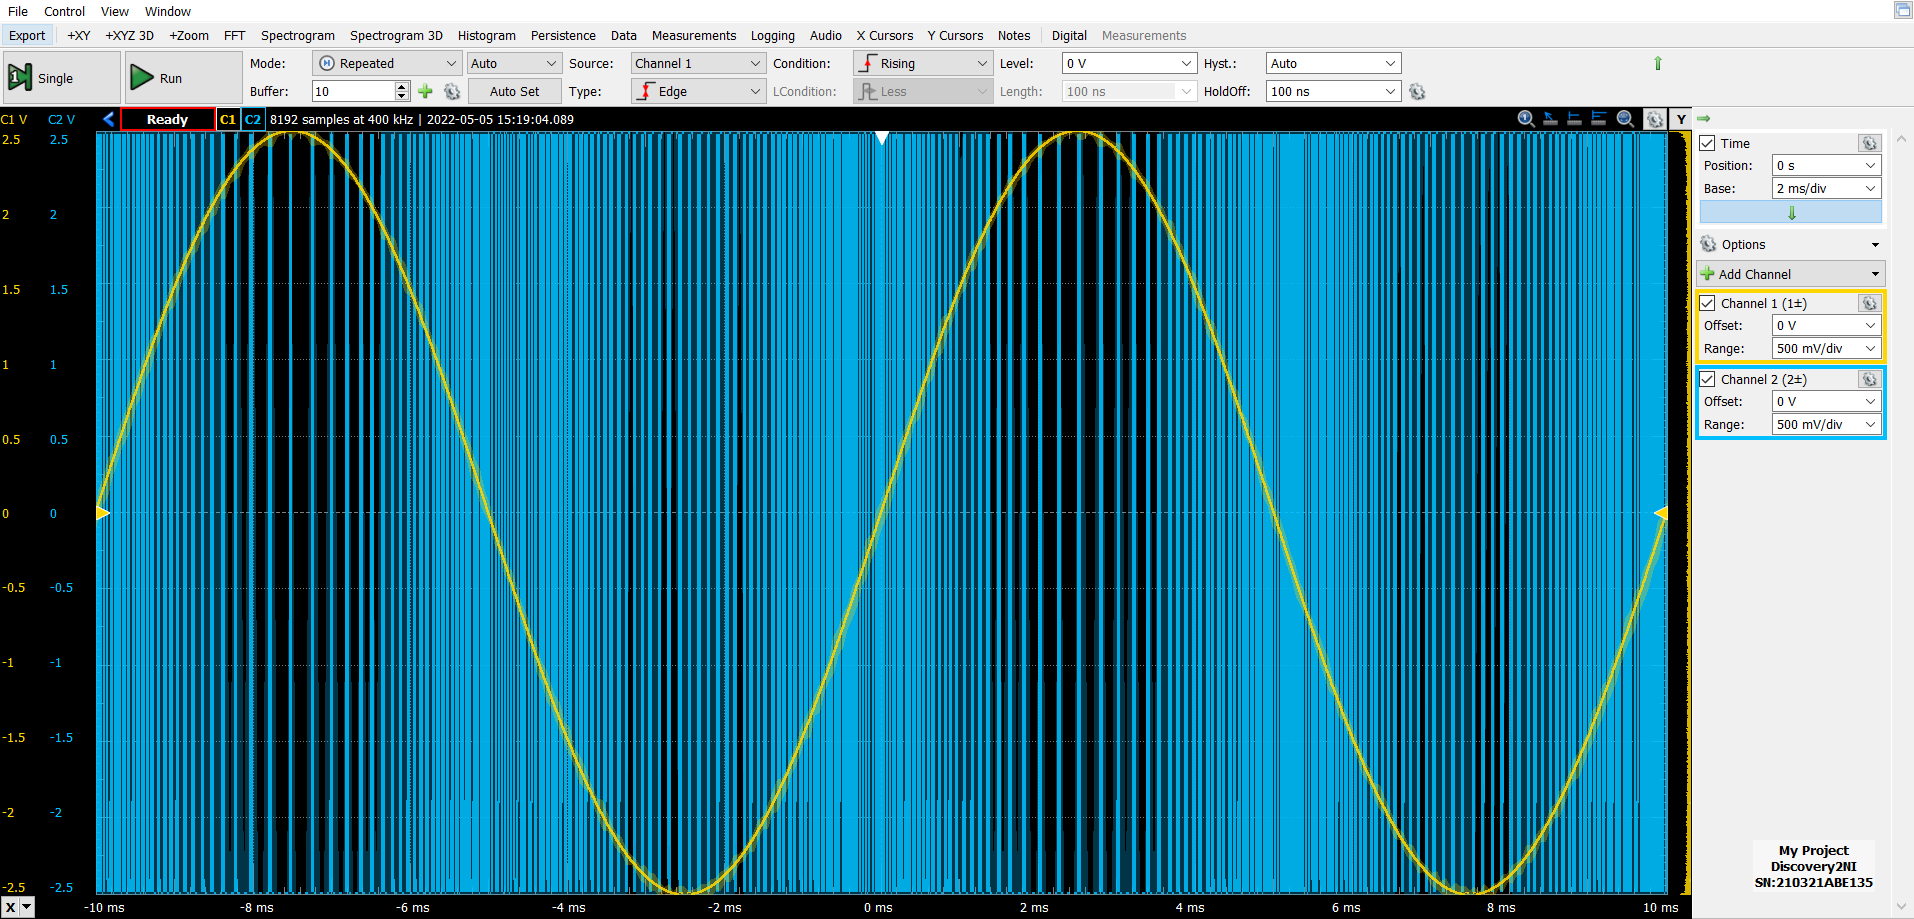
\includegraphics[width=\textwidth]{Conv.Sinusoide.100Hz.2}
    \caption{Acquisizione del segnale analogico in ingresso (un'onda sinusoidale di frequenza pari a 100 Hz e ampiezza pari a $2.5 V$) e del segnale in uscita dal DAC U4}
\end{figure}
%=======================
\section{Descrizione delle misure e acquisizione dati}

\subsection{Campionamento e acquisizione del segnale}

\subsection{Acquisizione con Protocol}

%=======================
\section{Analisi dei dati}

\subsection{Ricostruzione dei segnali in ingresso}

\subsection{Fit sinusoidale}

\subsection{Risposta in frequenza dell'ADC}

\subsection{Stima del fattore di calibrazione del convertitore}


\subsection{Misura del signal/noise ratio (SNR)}


%=======================
\section*{Conclusioni e commenti finali}
Si è riusciti a progettare, costruire e verificare il corretto funzionamento
di circuiti logici combinatori di diversa complessità e svariate applicazioni
(e.g., sistemi di controllo e misura) costruiti con porte NOT, NAND, OR e D-FF.
Inoltre si è riusciti ad apprezzare le diverse modalità di funzionamento delle
macchine a stati finiti implementate secondo i modelli Moore e Mealy, ponendo
particolare attenzione alle loro diverse temporizzazioni nei cambiamenti di
stato, nonostante la bassa risoluzione temporale dell'AD2.

%=======================
\section*{Dichiarazione}
I firmatari di questa relazione dichiarano che il contenuto della relazione \`e
originale, con misure effettuate dai membri del gruppo, e che tutti i firmatari
hanno contribuito alla elaborazione della relazione stessa.

\end{document}
\iffalse
⣿⣿⣿⣿⣿⣿⣿⣿⣿⣿⣿⣿⣿⣿⣿⣿⣿⣿⣿⣿⣿⣿⣿⣿⣿⣿⣿⣿⣿⣿⣿⣿⣿⣿⣿⣿⣿⣿⣿⣿⣿⣿⣿⣿⣿⣿⣿⣿⣿⣿
⣿⣿⣿⣿⣿⣿⣿⣿⣿⣿⣿⣿⣿⣿⣿⣿⣿⣿⣿⣿⣿⣿⣿⣿⣿⣿⣿⣿⣿⣿⣿⣿⣿⣿⣿⣿⣿⣿⣿⣿⣿⣿⣿⣿⣿⣿⣿⣿⣿⣿
⣿⣿⣿⣿⣿⣿⣿⣿⣿⣿⣿⣿⣿⣿⣿⣿⣿⣿⣿⣿⣿⣿⣿⣿⡿⢿⣿⣿⣿⣿⣿⣿⣿⣿⣿⣿⣿⣿⣿⣿⣿⣿⣿⣿⣿⣿⣿⣿⣿⣿
⣿⣿⣿⣿⣿⣿⣿⣿⣿⣿⣿⣿⣿⣿⣿⣿⣿⣿⣿⣿⣿⣿⣿⡟⠀⠀⢻⣿⣿⣿⣿⣿⣿⣿⣿⣿⣿⣿⣿⣿⣿⣿⣿⣿⣿⣿⣿⣿⣿⣿
⣿⣿⣿⣿⣿⣿⣿⣿⣿⣿⣿⣿⣿⣿⣿⣿⣿⣿⣿⣿⣿⣿⠟⠀⠐⠂⠀⠻⣿⣿⣿⣿⣿⣿⣿⣿⣿⣿⣿⣿⣿⣿⣿⣿⣿⣿⣿⣿⣿⣿
⣿⣿⣿⣿⣿⣿⣿⣿⣿⣿⣿⣿⣿⣿⣿⣿⣿⣿⣿⣿⣿⠏⠀⡠⠴⠤⣤⠀⠹⣿⣿⣿⣿⣿⣿⣿⣿⣿⣿⣿⣿⣿⣿⣿⣿⣿⣿⣿⣿⣿
⣿⣿⣿⣿⣿⣿⣿⣿⣿⣿⣿⣿⣿⣿⣿⣿⣿⣿⣿⣿⠏⠀⢀⣀⣀⣀⣀⡀⠀⠹⣿⣿⣿⣿⣿⣿⣿⣿⣿⣿⣿⣿⣿⣿⣿⣿⣿⣿⣿⣿
⣿⣿⣿⣿⣿⣿⣿⣿⣿⣿⣿⣿⣿⣿⣿⣿⣿⣿⡿⠃⠀⠈⠉⢁⣈⣿⣿⣿⣷⡀⠘⢿⣿⣿⣿⣿⣿⣿⣿⣿⣿⣿⣿⣿⣿⣿⣿⣿⣿⣿
⣿⣿⣿⣿⣿⣿⣿⣿⣿⣿⣿⣿⣿⣿⣿⣿⣿⡿⠃⠠⠴⠒⠛⠛⠛⠛⠛⠛⠛⠷⠄⠘⢿⣿⣿⣿⣿⣿⣿⣿⣿⣿⣿⣿⣿⣿⣿⣿⣿⣿
⣿⣿⣿⣿⣿⣿⣿⣿⣿⣿⣿⣿⣿⣿⣿⣿⡟⠁⠀⣀⣤⣴⣶⣶⣶⣶⣶⣶⣤⣄⣀⠀⠈⢻⣿⣿⣿⣿⣿⣿⣿⣿⣿⣿⣿⣿⣿⣿⣿⣿
⣿⣿⣿⣿⣿⣿⣿⣿⣿⣿⣿⣿⣿⣿⣿⠟⠀⣠⣾⣿⠿⠟⠛⠛⠛⠛⠛⠿⠿⣿⣿⣷⣆⠀⠻⣿⣿⣿⣿⣿⣿⣿⣿⣿⣿⣿⣿⣿⣿⣿
⣿⣿⣿⣿⣿⣿⣿⣿⣿⣿⣿⣿⣿⣿⠟⠀⠐⠋⠉⣀⡠⠤⠔⠒⠒⠒⠠⠤⢀⡀⠉⠛⠿⣆⠀⠻⣿⣿⣿⣿⣿⣿⣿⣿⣿⣿⣿⣿⣿⣿
⣿⣿⣿⣿⣿⣿⣿⣿⣿⣿⣿⣿⣿⠋⠀⢀⣠⠔⠊⠁⠀⢠⣤⣤⣶⣤⣤⣤⡀⠈⠑⠠⢄⠈⠁⠀⠙⣿⣿⣿⣿⣿⣿⣿⣿⣿⣿⣿⣿⣿
⣿⣿⣿⣿⣿⣿⣿⣿⣿⣿⣿⣿⠋⠀⢴⠋⠀⠀⠰⣧⠀⢸⣿⣿⣿⣿⣿⣿⡇⠀⣴⣄⠀⠑⠢⣤⡀⠙⣿⣿⣿⣿⣿⣿⣿⣿⣿⣿⣿⣿
⣿⣿⣿⣿⣿⣿⣿⣿⣿⣿⡿⠁⢀⣄⠀⠀⢾⣦⠀⠙⠦⠀⠙⠿⠿⠿⠿⠋⠀⣴⠋⠁⣀⣤⣠⣿⣷⡀⠈⢿⣿⣿⣿⣿⣿⣿⣿⣿⣿⣿
⣿⣿⣿⣿⣿⣿⣿⣿⣿⡟⠁⢀⠀⠙⢷⣶⣾⣿⣷⣤⣄⣰⣦⣄⣀⣀⣠⣴⣾⣿⣷⠾⠿⠀⠈⠉⠛⠓⠀⠈⢻⣿⣿⣿⣿⣿⣿⣿⣿⣿
⣿⣿⣿⣿⣿⣿⣿⣿⡟⠀⢀⠈⠓⢤⣀⠉⠙⠻⠿⠿⣿⣿⣿⣿⣿⣿⣿⣿⣿⣅⣀⣠⣤⣄⡀⠀⠒⠲⠶⠄⠀⢻⣿⣿⣿⣿⣿⣿⣿⣿
⣿⣿⣿⣿⣿⣿⣿⠏⠀⠀⠉⠀⠀⠀⠙⠷⣶⣤⣤⣀⣀⣀⡉⠉⣹⣿⣿⣿⣿⣿⣿⣿⣿⣿⣿⣶⣦⣤⣀⣀⣀⠀⠹⣿⣿⣿⣿⣿⣿⣿
⣿⣿⣿⣿⣿⣿⠏⠀⣰⣿⣷⣄⡀⠙⠢⡀⠈⠻⣿⣿⣿⣿⣿⣿⣿⣿⣿⣿⣿⣿⣿⣿⣿⣿⣿⣿⣿⣿⣿⣿⣿⣆⠀⠹⣿⣿⣿⣿⣿⣿
⣿⣿⣿⣿⣿⣇⣀⣀⣀⣀⣀⣀⣀⣀⣀⣀⣀⣀⣀⣀⣀⣀⣀⣀⣀⣀⣀⣀⣀⣀⣀⣀⣀⣀⣀⣀⣀⣀⣀⣀⣀⣀⣀⣀⣸⣿⣿⣿⣿⣿
⣿⣿⣿⣿⣿⣿⣿⣿⣿⣿⣿⣿⣿⣿⣿⣿⣿⣿⣿⣿⣿⣿⣿⣿⣿⣿⣿⣿⣿⣿⣿⣿⣿⣿⣿⣿⣿⣿⣿⣿⣿⣿⣿⣿⣿⣿⣿⣿⣿⣿
⣿⣿⣿⣿⣿⣿⣿⣿⣿⣿⣿⣿⣿⣿⣿⣿⣿⣿⣿⣿⣿⣿⣿⣿⣿⣿⣿⣿⣿⣿⣿⣿⣿⣿⣿⣿⣿⣿⣿⣿⣿⣿⣿⣿⣿⣿⣿⣿⣿⣿
⣿⣿⣿⣿⣿⣿⣿⣿⣿⣿⣿⣿⣿⣿⣿⣿⣿⣿⣿⣿⣿⣿⣿⣿⣿⣿⣿⣿⣿⣿⣿⣿⣿⣿⣿⣿⣿⣿⣿⣿⣿⣿⣿⣿⣿⣿⣿⣿⣿⣿
⣿⣿⣿⣿⣿⣿⣿⣿⣿⣿⣿⣿⣿⣿⣿⣿⣿⣿⣿⣿⣿⣿⣿⣿⣿⣿⣿⣿⣿⣿⣿⣿⣿⣿⣿⣿⣿⣿⣿⣿⣿⣿⣿⣿⣿⣿⣿⣿⣿⣿
⣿⣿⣿⣿⣿⣿⣿⣿⣿⣿⣿⣿⣿⣿⣿⣿⣿⣿⣿⣿⣿⣿⣿⣿⣿⣿⣿⣿⣿⣿⣿⣿⣿⣿⣿⣿⣿⣿⣿⣿⣿⣿⣿⣿⣿⣿⣿⣿⣿⣿
⣿⣿⣿⣿⣿⣿⠿⢋⣥⣴⣶⣶⣶⣬⣙⠻⠟⣋⣭⣭⣭⣭⡙⠻⣿⣿⣿⣿⣿
⣿⣿⣿⣿⡿⢋⣴⣿⣿⠿⢟⣛⣛⣛⠿⢷⡹⣿⣿⣿⣿⣿⣿⣆⠹⣿⣿⣿⣿
⣿⣿⣿⡿⢁⣾⣿⣿⣴⣿⣿⣿⣿⠿⠿⠷⠥⠱⣶⣶⣶⣶⡶⠮⠤⣌⡙⢿⣿
⣿⡿⢛⡁⣾⣿⣿⣿⡿⢟⡫⢕⣪⡭⠥⢭⣭⣉⡂⣉⡒⣤⡭⡉⠩⣥⣰⠂⠹
⡟⢠⣿⣱⣿⣿⣿⣏⣛⢲⣾⣿⠃⠄⠐⠈⣿⣿⣿⣿⣿⣿⠄⠁⠃⢸⣿⣿⡧
⢠⣿⣿⣿⣿⣿⣿⣿⣿⣇⣊⠙⠳⠤⠤⠾⣟⠛⠍⣹⣛⣛⣢⣀⣠⣛⡯⢉⣰
⣿⣿⣿⣿⣿⣿⣿⣿⣿⣿⣿⣿⣷⡶⠶⢒⣠⣼⣿⣿⣛⠻⠛⢛⣛⠉⣴⣿⣿
⣿⣿⣿⣿⣿⣿⣿⡿⢛⡛⢿⣿⣿⣶⣿⣿⣿⣿⣿⣿⣿⣿⣿⣿⣿⣷⡈⢿⣿
⣿⣿⣿⣿⣿⣿⣿⠸⣿⡻⢷⣍⣛⠻⠿⠿⣿⣿⣿⣿⣿⣿⣿⣿⣿⠿⢇⡘⣿
⣿⣿⣿⣿⣿⣿⣿⣷⣝⠻⠶⣬⣍⣛⣛⠓⠶⠶⠶⠤⠬⠭⠤⠶⠶⠞⠛⣡⣿
⢿⣿⣿⣿⣿⣿⣿⣿⣿⣿⣷⣶⣬⣭⣍⣙⣛⣛⣛⠛⠛⠛⠿⠿⠿⠛⣠⣿⣿
⣦⣈⠉⢛⠻⠿⠿⢿⣿⣿⣿⣿⣿⣿⣿⣿⣿⣿⣿⡿⠿⠛⣁⣴⣾⣿⣿⣿⣿
⣿⣿⣿⣶⣮⣭⣁⣒⣒⣒⠂⠠⠬⠭⠭⠭⢀⣀⣠⣄⡘⠿⣿⣿⣿⣿⣿⣿⣿
⣿⣿⣿⣿⣿⣿⣿⣿⣿⣿⣿⣿⣿⣿⣿⣿⣿⣿⣿⣿⣿⣦⡈⢿⣿⣿⣿⣿⣿
⠀⠀⠀⠀⠀⠀⠀⠀⠀⠀⠀⠀⠀⠀⠀⠀⠀⠀⠀⠀⠀⠀⠀⠀⠀⠀⠀⠀⠀⠀⠀⠀⠀⠀⣀⣀⣀⣀⣀⠀⠀⠀⠀⠀⠀⠀⠀⠀⠀⠀
⠀⠀⠀⠀⠀⠀⠀⠀⠀⠀⠀⠀⠀⠀⠀⠀⠀⠀⠀⠀⠀⠀⠀⠀⠀⠀⠀⠀⠀⠀⠀⠀⢀⣾⠋⠉⠉⠉⠙⠛⠻⢶⣤⡀⠀⠀⠀⠀⠀⠀
⠀⠀⠀⠀⠀⠀⠀⠀⠀⠀⠀⠀⠀⠀⠀⠀⠀⠀⠀⠀⠀⠀⠀⠀⠀⠀⠀⠀⠀⠀⠀⣠⡾⠁⠀⠀⠀⠀⠀⠀⠀⠀⠈⢻⡆⠀⠀⠀⠀⠀
⠀⠀⠀⠀⠀⠀⠀⠀⠀⠀⠀⠀⠀⠀⠀⠀⠀⠀⠀⠀⠀⠀⠀⠀⠀⠀⢀⣀⣀⣠⣴⠟⠀⠀⠀⠀⠀⠀⠀⠀⠀⠀⣠⡟⠁⠀⠀⠀⠀⠀
⠀⠀⠀⠀⠀⠀⠀⠀⠀⠀⠀⠀⠀⠀⠀⠀⠀⠀⠀⠀⠀⢀⣠⣴⠶⠟⠛⠉⠉⠁⠀⠀⠀⠀⠀⠀⠀⠀⠀⠀⠀⢰⡟⠀⠀⠀⠀⠀⠀⠀
⠀⠀⠀⠀⠀⠀⠀⠀⠀⠀⠀⠀⠀⠀⠀⠀⠀⣀⣠⣴⠾⠛⠉⠀⠀⠀⠀⠀⠀⠀⠀⠀⠀⠀⠀⠀⠀⠀⠀⠀⢀⣾⠁⠀⠀⠀⠀⠀⠀⠀
⠀⠀⠀⠀⠀⠀⠀⠀⠀⠀⠀⠀⠀⣠⡶⠛⠛⠋⠉⠀⠀⠀⠀⠀⠀⠀⠀⠀⠀⠀⠀⠀⠀⠀⠀⠀⠀⠀⠀⣴⠟⠁⠀⠀⠀⠀⠀⠀⠀⠀
⠀⠀⠀⠀⠀⠀⠀⠀⠀⠀⠀⠀⣰⡟⠀⠀⠀⠀⠀⠀⠀⠀⠀⠀⠀⠀⠀⠀⠀⠀⠀⠀⠀⠀⠀⠀⠀⢀⣾⠋⠀⠀⠀⠀⠀⠀⠀⠀⠀⠀
⠀⠀⠀⠀⠀⠀⠀⠀⠀⠀⣴⠞⠋⠀⠀⠀⠀⣠⣴⠶⠶⣦⡀⠀⠀⠀⠀⠀⠀⠀⠀⠀⠀⠀⠀⠀⣠⡿⠁⠀⠀⠀⠀⠀⠀⠀⠀⠀⠀⠀
⠀⠀⠀⠀⠀⠀⠀⠀⠀⠀⢿⣄⣀⣀⣤⡴⠟⠋⠀⠀⠀⠘⣷⡀⠀⠀⠀⠀⠀⠀⠀⠀⠀⠀⠀⣰⠟⠀⠀⠀⠀⠀⠀⠀⠀⠀⠀⠀⠀⠀
⠀⠀⠀⠀⠀⠀⠀⠀⠀⠀⢰⣟⠉⠙⢷⣄⠀⠀⠀⠀⠀⠀⠘⣷⠀⠀⠀⠀⠀⠀⠀⠀⠀⠀⣼⠏⠀⠀⠀⠀⠀⠀⠀⠀⠀⠀⠀⠀⠀⠀
⠀⠀⠀⠀⠀⠀⠀⠀⠀⠀⠀⠙⣷⡀⠀⠹⣧⡀⠀⠀⠀⠀⠀⣼⠃⠀⠀⠀⠀⠀⠀⠀⢀⣾⠃⠀⠀⠀⠀⠀⠀⠀⠀⠀⠀⠀⠀⠀⠀⠀
⠀⠀⠀⠀⠀⠀⠀⠀⠀⠀⠀⠀⠘⣷⡀⠀⠈⠛⣷⣤⣴⠶⠟⠃⠀⠀⠀⠀⠀⠀⠀⢀⣾⠃⠀⠀⠀⠀⠀⠀⠀⠀⠀⠀⠀⠀⠀⠀⠀⠀
⠀⠀⠀⠀⠀⠀⠀⠀⠀⠀⠀⠀⠀⠘⣷⡀⠀⠀⠈⠀⠀⠀⠀⠀⠀⠀⠀⠀⠀⠀⢀⣾⠃⠀⠀⠀⠀⠀⠀⠀⠀⠀⠀⠀⠀⠀⠀⠀⠀⠀
⠀⠀⠀⠀⠀⠀⠀⠀⠀⠀⠀⠀⠀⠀⠈⢷⣄⠀⠀⠀⠀⠀⠀⠀⠀⠀⠀⠀⠀⠀⢸⡇⠀⠀⠀⠀⠀⠀⠀⠀⠀⠀⠀⠀⠀⠀⠀⠀⠀⠀
⠀⠀⠀⠀⠀⠀⠀⠀⠀⠀⠀⠀⠀⠀⠀⠀⠙⠻⠟⠛⣻⡿⠀⠀⠀⠀⠀⢀⣤⡾⠛⠀⠀⠀⠀⠀⠀⠀⠀⠀⠀⠀⠀⠀⠀⠀⠀⠀⠀⠀
⠀⠀⠀⠀⠀⠀⠀⠀⠀⠀⠀⠀⠀⠀⠀⠀⠀⠀⣠⡾⠋⠀⠀⠀⠀⢀⣴⠟⣿⠀⠀⠀⠀⠀⠀⠀⠀⠀⠀⠀⠀⠀⠀⠀⠀⠀⠀⠀⠀⠀
⠀⠀⠀⠀⠀⠀⠀⠀⠀⠀⠀⠀⠀⠀⠀⠀⠀⣴⠟⠀⠀⠀⠀⣠⣾⡿⠁⢀⣿⠀⠀⠀⠀⠀⠀⠀⠀⠀⠀⠀⠀⠀⠀⠀⠀⠀⠀⠀⠀⠀
⠀⠀⠀⠀⠀⠀⠀⠀⠀⠀⠀⠀⠀⠀⠀⠀⣼⠏⠀⠀⠀⢀⡾⢫⣿⠁⠀⣼⠇⠀⠀⠀⠀⠀⠀⠀⠀⠀⠀⠀⠀⠀⠀⠀⠀⠀⠀⠀⠀⠀
⠀⠀⠀⠀⠀⠀⠀⠀⠀⠀⠀⠀⠀⠀⢀⡾⠃⠀⠀⢀⣴⠟⢡⡟⣿⠀⠀⣿⠀⠀⠀⠀⠀⠀⠀⠀⠀⠀⠀⠀⠀⠀⠀⠀⠀⠀⠀⠀⠀⠀
⠀⠀⠀⠀⠀⠀⠀⠀⠀⠀⠀⠀⠀⣰⠟⠁⠀⠀⣰⠟⠁⢠⡿⠀⢿⡄⢰⡟⠀⠀⠀⠀⠀⠀⠀⠀⠀⠀⠀⠀⠀⠀⠀⠀⠀⠀⠀⠀⠀⠀
⠀⠀⠀⠀⠀⠀⠀⠀⠀⠀⠀⠀⣼⠏⠀⠀⢠⣾⠋⠀⢀⡿⠁⠀⠈⠛⠿⠃⠀⠀⠀⠀⠀⠀⠀⠀⠀⠀⠀⠀⠀⠀⠀⠀⠀⠀⠀⠀⠀⠀
⠀⠀⠀⠀⠀⠀⠀⠀⠀⠀⠀⢸⡏⠀⠀⣴⢿⡟⠀⠀⣾⠃⠀⠀⠀⠀⠀⠀⠀⠀⠀⠀⠀⠀⠀⠀⠀⠀⠀⠀⠀⠀⠀⠀⠀⠀⠀⠀⠀⠀
⠀⠀⠀⠀⠀⠀⠀⠀⠀⠀⠀⠈⢷⣄⣾⠋⠘⣧⡀⢰⡟⠀⠀⠀⠀⠀⠀⠀⠀⠀⠀⠀⠀⠀⠀⠀⠀⠀⠀⠀⠀⠀⠀⠀⠀⠀⠀⠀⠀⠀
⠀⠀⠀⠀⠀⠀⠀⠀⠀⠀⠀⠀⠀⠉⠁⠀⠀⠈⠛⠋⠀⠀⠀⠀⠀⠀⠀⠀⠀⠀⠀⠀⠀⠀⠀⠀⠀⠀⠀⠀⠀⠀⠀⠀⠀⠀⠀⠀⠀⠀
⠀⠀⠀⠀⠀⠀⠀⠀⠀⠀⠀⠀⠀⠀⠀⠀⠀⠀⠀⠀⠀⠀⢀⡤⠶⢶⣶⣦⣄⡀⠀⠀
⠀⠀⠀⠀⠀⠀⠀⠀⠀⠀⠀⠀⠀⠀⠀⠀⠀⠀⠀⠀⠀⣠⣾⣿⡄⠒⠪⢝⠻⣿⣿⣦⡀
⠀⠀⠀⠀⠀⠀⠀⠀⠀⠀⠀⠀⠀⠀⠀⠀⠀⠀⠀⠀⣴⣿⡿⢉⡀⠀⠈⠐⠄⢿⣿⣿⣷
⠀⠀⠀⠀⠀⠀⠀⠀⠀⠀⠀⠀⠀⠀⠀⠀⠀⠀⠀⣼⣿⡇⠀⠀⠈⡄⠤⢀⠈⣾⣿⣿⣿
⠀⠀⠀⠀⠀⠀⠀⠀⠀⠀⠀⠀⠀⠀⠀⠀⠀⢀⡾⣿⣟⣕⡤⡠⠘⠀⠀⠀⢱⣿⣿⣿⣿
⠀⠀⠀⠀⠀⠀⠀⠀⠀⠀⠀⠀⠀⠀⠀⠀⢠⣾⣾⣿⣞⣄⠮⠔⠈⡢⠄⣠⣾⣿⣿⣿⣿
⠀⠀⠀⠀⠀⠀⠀⠀⠀⠀⠀⠀⠀⠀⠀⠠⢿⣿⢽⡻⣿⣿⣿⣽⣵⣾⡽⣿⣿⣿⣿⣿⡏
⠀⠀⠀⠀⠀⠀⠀⠀⠀⠀⠀⠀⠀⠀⢠⣗⣿⡟⠈⠉⠚⢽⣻⢷⡝⣿⡿⣿⣿⣿⣿⡿⠀
⠀⠀⠀⠀⠀⠀⠀⠀⠀⠀⠀⠀⠀⢠⣿⣿⣿⠇⠀⠀⠀⠀⠀⢩⣯⣭⣾⣿⣿⣿⣿⠁⠀
⠀⠀⠀⠀⠀⠀⠀⠀⠀⠀⠀⠀⣰⣿⣿⣿⠃⠀⠀⠀⠀⠀⣰⣿⣿⣿⣿⣿⣿⣿⠃⠀⠀
⠀⠀⠀⠀⠀⠀⠀⠀⠀⠀⠀⣴⣿⣿⡿⠃⠀⠀⠀⠀⣠⣼⣿⣿⣿⣿⣿⣿⣿⠃⠀⠀⠀
⠀⠀⠀⠀⠀⠀⠀⠀⠀⢀⢞⣿⣿⡿⠁⠀⠀⠀⣠⣾⣿⣿⣿⣿⣿⣿⣿⣿⠃⠀⠀⠀⠀
⠀⠀⠀⠀⠀⠀⠀⠀⣰⣿⣾⣿⠏⠀⠀⠀⠀⣾⣿⣿⣿⣿⣿⣿⡟⣿⣿⠏⠀⠀⠀⠀⠀
⠀⠀⠀⠀⠀⠀⣠⣾⣿⣿⣿⠃⠀⠀⠀⠀⣸⣿⣿⣿⣿⣿⣟⣷⣾⣿⠏⠀⠀⠀⠀⠀⠀
⠀⠀⠀⠀⢀⣾⣿⣿⣿⣿⠃⠀⠀⠀⢀⣴⣿⣿⣿⣿⣿⣿⣿⣿⣿⠋⠀⠀⠀⠀⠀⠀⠀
⠀⠀⠀⡰⢿⣿⣿⣯⡶⠁⠀⠀⢀⣴⣿⣿⣿⣿⣿⣿⣿⣿⣿⡿⠃⠀⠀⠀⠀⠀⠀⠀⠀
⠀⢀⣼⣟⣿⣿⡿⠃⠀⠀⢀⣴⣿⣿⣿⣿⣿⣿⣿⣿⣿⣿⡟⠁⠀⠀⠀⠀⠀⠀⠀⠀⠀
⢀⣾⣿⣿⡯⣿⠀⠀⢠⣴⣿⣿⣿⣿⣿⣿⣿⣿⣿⣿⣿⠏⠀⠀⠀⠀⠀⠀⠀⠀⠀⠀⠀⠀⠀
⣾⣿⣿⣿⣿⣿⣶⣶⣿⣿⣿⣿⣿⣿⣿⣿⣿⣿⣿⡿⠁⠀⠀⠀⠀⠀⠀⠀⠀⠀⠀⠀⠀
⠿⣿⡿⣿⣿⣿⣿⣿⣿⣿⣿⣿⣿⣿⣿⣿⢿⡿⠋⠀⠀⠀⠀⠀⠀⠀⠀⠀⠀⠀⠀⠀⠀
⠀⠛⠀⠈⠀⠻⣿⣿⣿⣿⣿⣟⣛⣿⣿⡭⠋⠀⠀⠀⠀⠀⠀⠀⠀⠀⠀⠀⠀⠀⠀⠀⠀
⠢⡀⠀⠀⠀⠀⠻⣿⣿⣿⣿⣿⣭⠟⠉⠀⠀⠀⠀⠀⠀⠀⠀⠀⠀⠀⠀⠀⠀⠀⠀⠀⠀
⠀⠈⠐⠤⢀⡀⠀⢀⣙⣿⠿⠋⠁⠀⠀⠀⠀⠀⠀⠀⠀⠀⠀⠀⠀⠀⠀⠀⠀⠀⠀⠀⠀
⠀⠀⠀⠀⠀⠀⠀⠀⠀⠀⠀⠀⠀⠀⠀⠀⠀⠀⠀⠀⠀⠀⠀⠀
⣿⣿⣿⣿⣿⣿⣿⣿⣿⣿⣿⣿⣿⣿⣿⡿⠿⠛⠛⠛⠛⠿⣿⣿⣿⣿⣿⣿⣿⣿
⣿⣿⣿⣿⣿⣿⣿⣿⣿⣿⣿⡿⠛⠉⠁⠀⠀⠀⠀⠀⠀⠀⠉⠻⣿⣿⣿⣿⣿⣿
⣿⣿⣿⣿⣿⣿⣿⣿⣿⣿⡟⠁⠀⠀⠀⠀⠀⠀⠀⠀⠀⠀⠀⠀⠘⢿⣿⣿⣿⣿
⣿⣿⣿⣿⣿⣿⣿⣿⣿⡟⠁⠀⠀⠀⠀⠀⠀⠀⠀⠀⠀⠀⠀⠀⠀⣾⣿⣿⣿⣿
⣿⣿⣿⣿⣿⣿⣿⠋⠈⠀⠀⠀⠀⠐⠺⣖⢄⠀⠀⠀⠀⠀⠀⠀⠀⣿⣿⣿⣿⣿
⣿⣿⣿⣿⣿⣿⡏⢀⡆⠀⠀⠀⢋⣭⣽⡚⢮⣲⠆⠀⠀⠀⠀⠀⠀⢹⣿⣿⣿⣿
⣿⣿⣿⣿⣿⣿⡇⡼⠀⠀⠀⠀⠈⠻⣅⣨⠇⠈⠀⠰⣀⣀⣀⡀⠀⢸⣿⣿⣿⣿
⣿⣿⣿⣿⣿⣿⡇⠁⠀⠀⠀⠀⠀⠀⠀⠀⠀⠀⠀⣟⢷⣶⠶⣃⢀⣿⣿⣿⣿⣿
⣿⣿⣿⣿⣿⣿⡅⠀⠀⠀⠀⠀⠀⠀⠀⠀⠀⠀⠀⢿⠀⠈⠓⠚⢸⣿⣿⣿⣿⣿
⣿⣿⣿⣿⣿⣿⡇⠀⠀⠀⠀⢀⡠⠀⡄⣀⠀⠀⠀⢻⠀⠀⠀⣠⣿⣿⣿⣿⣿⣿
⣿⣿⣿⣿⣿⣿⡇⠀⠀⠀⠐⠉⠀⠀⠙⠉⠀⠠⡶⣸⠁⠀⣠⣿⣿⣿⣿⣿⣿⣿
⣿⣿⣿⣿⣿⣿⣿⣦⡆⠀⠐⠒⠢⢤⣀⡰⠁⠇⠈⠘⢶⣿⣿⣿⣿⣿⣿⣿⣿⣿
⣿⣿⣿⣿⣿⣿⣿⣿⡇⠀⠀⠀⠀⠠⣄⣉⣙⡉⠓⢀⣾⣿⣿⣿⣿⣿⣿⣿⣿⣿
⣿⣿⣿⣿⣿⣿⣿⣿⣷⣄⠀⠀⠀⠀⠀⠀⠀⠀⣰⣿⣿⣿⣿⣿⣿⣿⣿⣿⣿⣿
⣿⣿⣿⣿⣿⣿⣿⣿⣿⣿⣷⣤⣀⣀⠀⣀⣠⣾⣿⣿⣿⣿⣿⣿⣿⣿⣿⣿⣿⣿
⣿⣿⣿⣿⣿⣿⣿⣿⣿⣿⣿⣿⣿⣿⣿⣿⣿⣿⣿⣿⣿⣿⣿⣿⣿⣿⣿⣿⣿⣿
⣿⣿⣿⣿⣿⣿⣿⣿⣿⣿⠿⠟⠋⠉⠉⠉⠙⠛⠻⠿⣿⣿⣿⣿⣿⣿⣿⣿⣿⣿
⣿⣿⣿⣿⣿⣿⣿⣿⠟⠁⠀⠀⠀⠀⠀⣠⣤⣦⣤⡀⠈⠻⣿⣿⣿⣿⣿⣿⣿⣿
⣿⣿⣿⣿⣿⣿⣿⠏⠀⠀⠀⠀⣴⣶⣿⣿⣿⣿⣿⣿⣷⡄⠘⣿⣿⣿⣿⣿⣿⣿
⣿⣿⣿⣿⣿⣿⡿⠀⣼⠀⠀⢨⣿⣿⣿⣿⣿⣿⣿⣿⣿⣷⡘⢿⣿⣿⣿⣿⣿⣿
⣿⣿⣿⣿⣿⣿⣿⡏⡄⠄⠀⠘⣿⣿⣿⣿⣿⣿⣿⣿⣿⣿⣿⣝⣿⣿⣿⣿⣿⣿
⣿⣿⣿⣿⣿⡟⠺⢰⣦⡄⠀⠠⠙⢿⣿⣿⣿⣿⣿⣿⣿⣿⣿⣿⡽⣿⣿⣿⣿⣿
⣿⣿⣿⣿⣿⣧⠀⢸⡋⠀⠀⠀⠀⠀⢹⣯⡀⠀⠠⣈⣿⣿⣿⣿⣿⣿⣿⣿⣿⣿
⣿⣿⣿⣿⣿⣿⡇⢺⠇⠀⣬⣶⡇⠀⢸⣿⣿⣿⣿⣿⣿⣿⣿⣿⣿⣿⣿⣿⣿⣿
⣿⣿⣿⣿⣿⣿⣷⡈⠀⠀⠈⢻⠋⠀⢸⣿⣿⣿⣿⣿⣿⣿⣿⣿⣿⣿⣿⣿⣿⣿
⣿⣿⣿⣿⣿⣿⣿⣿⠀⠀⠀⠀⠀⠀⠘⢿⣻⣿⣿⣿⣿⣿⣿⣿⣿⣿⣿⣿⣿⣿
⣿⣿⣿⣿⣿⣿⣿⣿⡀⠀⠀⠀⠀⠀⠴⠸⠿⠿⢿⣿⣿⣿⣿⣿⣿⣿⣿⣿⣿⣿
⣿⣿⣿⣿⣿⣿⣿⣿⢳⡀⠀⠀⠀⠀⣈⣈⣽⣿⣶⣿⣟⣿⣿⣿⣿⣿⣿⣿⣿⣿
⣿⣿⣿⣿⣿⣿⠟⠁⠘⣷⣤⡀⠀⠀⠐⠙⠛⠛⣩⣵⣿⠻⣿⣿⣿⣿⣿⣿⣿⣿
⣿⡿⠿⠛⠉⠁⠀⠀⠀⠈⢿⣿⣶⣄⣤⣤⣐⣾⣿⣿⣿⡆⠈⠻⠿⣿⣿⣿⣿⣿
⠁⠀⠀⠀⠀⠀⠀⠀⠀⠀⠈⢿⣿⣿⣿⣿⣿⠿⠿⣿⣿⣧⠀⠀⠀⠀⠈⠉⠛⠿
⠀⠀⠀⠀⠀⠀⠀⠀⠀⠀⠀⠘⣿⣿⣿⡟⠁⠀⠀⠈⢹⣿⣇⠀⠀⠀⠀⠀⠀⠀
⠀⠀⠀⠀⠀⠀⠀⠀⠀⠀⠀⠀⠘⣿⣿⣷⣦⣀⠀⠀⣿⣿⣿⠀⠀⠀⠀⠀⠀⠀
⠀⠀⠀⠀⠀⠀⠀⠀⠀⠀⠀⠀⠀⢹⣿⣿⣿⡟⠀⠈⢹⣿⣿⡇⠀⠀⠀⠀⠀⠀
⠀⠀⠀⠀⠀⠀⠀⠀⠀⠀⠀⠀⠀⠀⢻⣿⣿⠃⠀⠀⠸⣿⣿⣷⠀⠀⠀⠀⠀⠀
⠀⠀⠀⠀⠀⠀⠀⠀⠀⠀⠀⠀⠀⠀⠈⢿⣿⠀⠀⠀⠀⢻⣿⣿⠀⠀⠀⠀⠀⠀
⠀⠀⠀⠀⠀⠀⠀⠀⠀⠀⠀⠀⠀⠀⠀⠈⣿⠀⠀⠀⠀⠈⢿⣿⡇⠀⠀⠀⠀⠀
⠄⠄⠄⠄⠄⠄⠄⠄⠄⠄⠄⠄⠄⠄⠄⠄⢀⠄⡀⠄⡀⢀⠄⡀⡀⠠⢀⠄⠄⠄⠄⠄⠄⠄⠄⠄⠄⠄⠄⠄⠄⠄⠄⠄⠄⠄
⠄⠄⠄⠄⠄⠄⠄⠄⠄⠄⠄⠄⠄⠄⠄⡀⠠⢀⠄⡅⢔⠰⡨⢢⢡⢑⠔⠅⠕⠄⠅⠄⠄⠄⠄⠄⠄⠄⠄⠄⠄⠄⠄⠄⠄⠄
⠄⠄⠄⠄⠄⠄⠄⠄⠄⠄⠄⠄⠄⡀⠅⢔⠨⢐⠅⡌⢆⢣⠪⡪⡘⡌⡮⡱⡡⣊⢌⢀⢀⠄⠄⠄⠄⠄⠄⠄⠄⠄⠄⠄⠄⠄
⠄⠄⠄⠄⠄⠄⠄⠄⠄⠄⠄⠠⡐⢄⠕⡡⡘⢔⢱⢨⢪⢪⢪⢪⡺⣪⢞⢮⢫⢮⢺⢔⢆⡢⠄⠄⠄⠄⠄⠄⠄⠄⠄⠄⠄⠄
⠄⠄⠄⠄⠄⢀⠐⠈⠄⡠⡊⢌⠢⡑⡌⡆⡇⡇⡇⡇⣇⢗⣝⢮⡺⣪⡳⣹⡪⣞⢵⢝⡵⡝⣕⠡⢀⢂⠄⠄⠄⠄⠄⠄⠄⠄
⠄⠄⠄⠄⢠⢊⢂⠁⡔⡌⡢⢑⠌⡢⡱⡸⡸⡸⡪⡺⡸⣕⢵⡳⣝⢮⡺⣪⢞⣵⣫⡳⣕⢯⡺⡬⠄⠕⡕⡄⠄⠄⠄⠄⠄⠄
⠄⠄⠄⠄⡇⡇⡂⢢⢣⢣⠨⡂⡊⢔⢕⢱⡱⡝⣜⢝⡺⣜⡵⣝⢮⡳⡽⣵⣻⡺⣼⡺⡵⣳⢝⡮⡃⡕⡺⢄⠄⠄⠄⠄⠄⠄
⠄⠄⠄⢸⡱⡱⡨⢪⢪⢢⠡⢂⢊⠢⡱⡱⡱⡝⡮⡳⣝⢞⢮⢗⡯⣯⢯⣗⡯⣟⣮⢯⣟⢮⡳⣝⢇⢇⢎⢵⡀⠄⠄⠄⠄⠄
⠄⠄⠄⣕⢵⢣⢣⢑⢅⢆⢃⠢⠡⡡⡱⡱⡹⡪⡯⣺⢕⡯⣫⢯⢾⢽⢽⣺⢯⣗⡯⣗⣗⢗⣝⢮⡫⣏⢮⢒⢅⠄⠄⠄⠄⠄
⠄⠄⢀⠮⡪⢪⠪⠢⡃⡪⡂⠅⢕⠰⢱⢸⢸⡱⣝⢮⡳⡽⣪⢏⡯⡯⣟⡾⣽⣺⢽⣳⡳⣝⢮⡳⣫⣳⢳⡱⡱⠄⠄⠄⠄⠄
⠄⠄⢀⡃⡫⢔⢨⢕⢕⢔⢌⢌⠢⡑⡱⡘⢜⢜⢮⡳⣝⣞⢵⣫⢿⢽⣺⡽⡾⣾⢽⣳⢯⢮⡳⣝⣕⢗⢵⡑⡕⡀⠄⠄⠄⠄
⠄⠄⠐⠢⡱⡐⢕⢵⣑⡑⢕⢐⠕⠸⠰⡑⠕⢕⢕⠽⡕⣏⢗⢽⢝⢽⠺⠽⠽⢽⢻⢽⢽⢵⢽⡸⣪⢳⢱⢱⡱⡽⡡⡀⠄⠄
⠄⠄⠨⠈⢆⢊⢎⢖⢂⠃⠡⠐⠈⠈⠄⠄⠄⠄⠄⢑⢹⢘⣜⢕⠑⡈⠄⡈⣈⣐⠨⠘⡜⢕⡳⣝⢮⡳⡱⡱⡵⡯⡪⠂⠄⠄
⠄⠄⠄⠅⢂⠑⡕⡕⠄⡢⢀⠄⠠⠄⠁⠁⡌⠠⢠⠄⠸⣸⣺⡪⣐⠅⢢⢈⠄⢬⢍⣆⢧⣳⡽⡮⣺⡪⡺⣘⢼⣝⠆⠄⠄⠄
⠄⠄⠄⠨⡢⡢⡣⡳⢑⢰⢐⠠⡊⡪⣢⡣⡪⡰⠑⡀⠨⣪⢷⣝⡮⡫⡪⣪⢾⢝⣯⢾⣝⣗⡯⣟⢮⡪⡯⡷⣗⡯⠄⠄⠄⠄
⠄⠄⠄⠄⢕⠄⡇⡣⡑⠔⢅⠇⡇⡏⡖⡕⡕⣌⢂⠂⠌⢮⢷⡳⡯⡯⡾⡵⣫⢯⢞⣗⡷⡯⣯⡳⣱⢱⢝⡽⣺⠁⠄⠄⠄⠄
⠄⠄⠄⠄⠡⡡⢱⢐⠨⠨⠐⡡⢃⢇⢇⡏⡞⡔⡐⠠⢑⢽⢽⢽⢽⢽⢽⣝⢗⡯⣟⢾⢽⢝⡞⣜⢜⢜⣽⣺⠎⠄⠄⠄⠄⠄
⠄⠄⠄⠄⠄⠊⠃⠂⡐⠄⠅⡐⡈⡢⡃⢇⠕⡢⠄⠨⢘⢮⢯⢯⣳⡫⡗⣗⢽⢝⡮⡯⡮⡣⡏⣎⢎⠞⠺⠊⠄⠄⠄⠄⠄⠄
⠄⠄⠄⠄⠄⠄⠄⠄⠂⡁⢂⠐⡈⡢⢑⠅⡕⡐⠈⠨⡨⢯⣻⢽⣺⢺⡺⡪⣏⢷⢽⢕⣯⡫⣞⢜⢜⠄⠄⠄⠄⠄⠄⠄⠄⠄
⠄⠄⠄⠄⠄⠄⠄⠄⡁⠄⠄⠂⡂⠌⠄⢕⢐⠌⢄⠄⠨⠨⢘⢥⢅⡵⣝⣝⢮⡳⡽⣝⡮⣺⢪⢎⣗⠄⠄⠄⠄⠄⠄⠄⠄⠄
⠄⠄⠄⠄⠄⠄⠄⠄⠄⢂⢀⠡⠄⠌⠌⢂⢂⠪⠐⡌⢰⢰⢘⢼⢝⣞⢞⣞⡵⡯⣞⢵⣫⢮⡳⡣⡳⠄⠄⠄⠄⠄⠄⠄⠄⠄
⠄⠄⠄⠄⠄⠄⠄⠄⠈⡀⠐⠄⠊⠄⠨⠐⠠⠈⠌⠘⠜⠵⡢⢳⢹⢜⢕⠕⠱⡹⡪⡳⣕⣳⢹⡸⠅⠄⠄⠄⠄⠄⠄⠄⠄⠄
⠄⠄⠄⠄⠄⠄⠄⠄⠄⠄⠈⢄⠡⠁⠠⠄⠄⡀⠄⠐⠔⠔⠔⡢⠦⣒⢎⣎⢦⢢⢩⡫⣎⢮⢣⠃⠄⠄⠄⠄⠄⠄⠄⠄⠄⠄
⠄⠄⠄⠄⠄⠄⠄⠄⢰⣇⠄⠐⠠⠄⠁⠄⠡⢀⢂⢅⢔⢄⣆⣆⢕⢵⡹⣪⡳⣕⢵⢱⢕⢇⡇⠄⠄⠄⠄⠄⠄⠄⠄⠄⠄⠄
⠄⠄⠄⠄⠄⠄⠄⠄⠱⡿⣵⣀⠄⠄⠄⠈⠨⠨⡂⢇⢎⢕⢎⢞⡽⡵⣝⢮⢺⢸⠸⡘⣜⢼⠄⠄⠄⠄⠄⠄⠄⠄⠄⠄⠄⠄
⠄⠄⠄⠄⠄⠄⠄⠄⠄⢹⣺⣳⣧⣄⡀⠄⠄⡀⠂⠌⡂⠕⢌⠊⢎⠪⠪⠪⡊⡆⣕⣕⢧⣓⣧⠄⠄⠄⠄⠄⠄⠄⠄⠄⠄⠄
⠄⠄⠄⠄⠄⠄⠄⠄⠄⠈⢪⢞⣾⡽⣷⣮⡄⠐⠄⡂⠌⢌⠢⢑⢐⢄⢅⢇⢇⣗⣕⢗⡵⣽⣿⠄⠄⠄⠄⠄⠄⠄⠄⠄⠄⠄
⠄⠄⠄⠄⠄⠄⠄⠄⠄⠄⠄⠙⡾⣽⣯⣷⣿⡿⣮⣰⢱⡱⣜⢔⡑⡜⣜⢮⣣⡳⣪⢷⣽⣿⣿⡀⠄⠄⠄⠄⠄⠄⠄⠄⠄⠄
⠄⠄⠄⠄⠄⠄⠄⠄⠄⠄⠄⠄⠘⡷⣿⣽⣿⣿⣿⣿⣿⣾⣮⣗⣽⢵⢕⣕⢮⡺⢝⣵⣿⣿⣿⣷⠄⠄⠄⠄⠄⠄⠄⠄⠄⠄
⠄⠄⠄⠄⠄⠄⠄⠄⠄⠄⠄⠄⠄⠘⣯⡿⣿⣿⣿⣿⣿⣿⣿⣿⣿⣿⣷⣵⣏⣾⣿⣿⣿⣿⣿⣿⣇⠄⠄⠄⠄⠄⠄⠄⠄⠄
⠄⠄⠄⠄⠄⠄⠄⠄⠄⠄⠄⠄⠄⠄⠻⣟⣿⣿⣿⣿⣿⣿⣿⣿⣿⠏⠉⠄⠄⠄⠉⠻⢿⣿⣿⣿⣿⡀⠄⠄⠄⠄⠄⠄⠄⠄
⠄⠄⠄⠄⠄⠄⠄⠄⠄⠄⠄⠄⠄⠄⠄⢻⣿⣿⣿⣿⣿⣿⣿⡟⠁⠄⠄⠁⠠⠄⠄⠄⠈⠽⣿⣿⣿⣷⠄⠄⠄⠄⠄⠄⠄⠄
⠄⠄⠄⠄⠄⠄⠄⠄⠄⠄⠄⠄⠄⠄⠄⠈⢿⣿⣿⣿⣿⣿⡵⣄⠄⠄⠄⠄⠁⠈⠄⠄⢸⣹⡪⣿⣿⣿⡂⠄⠄⠄⠄⠄⠄⠄
⠄⠄⠄⠄⠄⠄⠄⠄⠄⠄⠄⠄⠄⠄⠄⠄⠈⢿⣿⣿⣻⣿⣿⣯⣿⣢⣄⠄⠄⠄⠑⠠⢸⣿⣿⣮⢞⣿⣧⠄⠄⠄⠄⠄⠄⠄
\fi